\chapter{小脑} \label{chap:chap37}

小脑仅占大脑总体积的 10\%,但包含一半以上的神经元。
小脑皮层由一系列高度规则的重复单元组成,每个单元都包含相同的基本微回路。
小脑的不同区域接收来自不同大脑和脊柱结构的投射,然后投射回大脑。
小脑所有区域的结构和生理学的相似性意味着小脑的不同区域对不同的输入执行相似的计算操作。


人类和实验动物的小脑损伤症状提供了令人信服的证据,证明小脑参与了对运动的控制。
因此,这些症状除了可以为临床医生提供诊断外,还有助于确定小脑在控制行为中的可能作用。


几个基本原则定义了我们对小脑生理功能的理解。
首先,小脑在运动产生的感觉反馈之前起作用,从而提供肌肉收缩的前馈控制。
其次,为了实现这种控制,小脑依靠身体的内部模型来处理感觉输入并将其与运动命令的副本进行比较。
第三,小脑在运动和知觉时间上起着特殊的作用。
第四,小脑对于适应和学习运动技能至关重要。
最后,灵长类动物的小脑与大脑皮层的非运动区域有广泛的联系,表明它在运动和非运动行为的表现和学习中发挥着相似的功能。


% 参考:https://www.dxy.cn/bbs/newweb/pc/post/40268362

\section{小脑损伤导致明显的症状和体征}

\subsection{损伤导致运动和姿势的特征性异常}

涉及小脑的疾病通常会破坏正常的运动模式,证明小脑在运动中的关键作用。
患者描述失去了大多数动作的自动、无意识的性质。
20世纪初,戈登·霍姆斯记录了一位右小脑半球受损男子的自述:“我左臂的动作是下意识的,但右臂的每一个动作我都得考虑。
我在转弯时突然停了下来,在我重新开始之前必须考虑一下。”


这被解释为小脑输入和输出的自动处理水平中断。
由于小脑功能障碍,大脑皮层似乎需要在编程运动动作的细节方面发挥更积极的作用。
重要的是,患有小脑损伤的个体不会经历与大脑皮层损伤相关的麻痹。
相反,他们在自主运动、行走和姿势方面表现出特征性异常,这些异常提供了有关小脑功能的重要线索。


小脑障碍最突出的症状是共济失调,或运动不协调。
共济失调是一个通用术语,用于描述与小脑损伤相关的集体运动特征。
患有小脑疾病的人做出的运动在性质上显得生涩、不规则且高度可变。 
到达期间的肢体共济失调的特征是弯曲的手部路径不对称,因为它们超过或低于预期目标并振荡(图~\ref{fig:37_1}A)。
患者经常将运动分解成多个部分,大概是为了简化对多关节运动的控制(运动分解)。
然而,这可能并不有效。
例如,患者在移动肘部时通常难以保持肩部稳定,这种缺陷被认为是由于对肘部运动如何机械影响肩部的预测不佳所致(图~\ref{fig:37_1}B)。
如果预测失败,则患者将被迫尝试使用延时反馈来稳定肩部,但效果较差。


\begin{figure}[htbp]
	\centering
	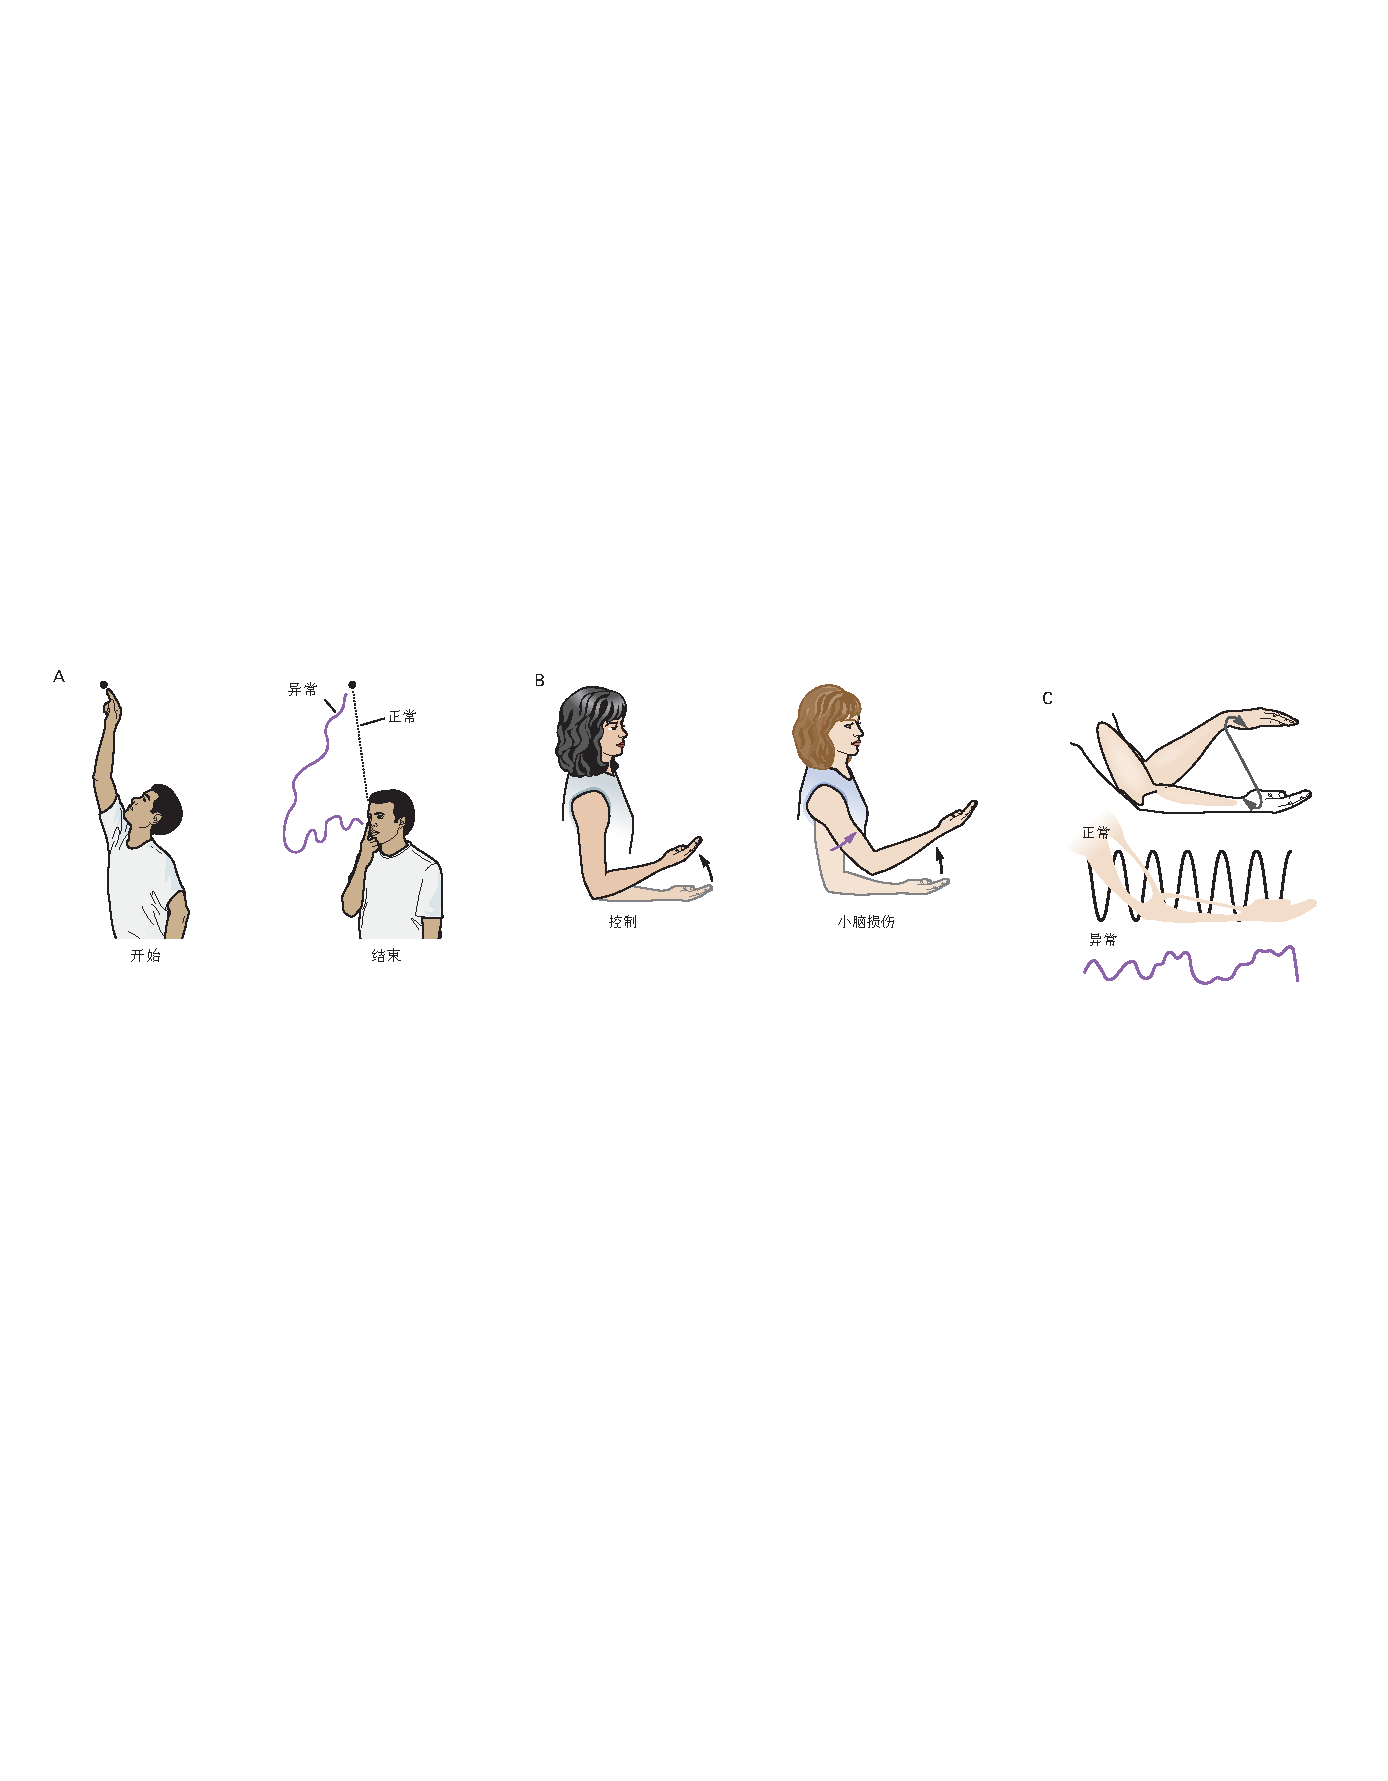
\includegraphics[width=0.85\linewidth]{chap37/fig_37_1}
	\caption{在小脑疾病中观察到的典型缺陷。
		\textbf{A.} 一位小脑患者将他的手臂从抬高的位置移动到触摸他的鼻尖显示出范围和方向不准确(辨距障碍)并且分开移动他的肩膀和肘部(运动分解)。 
		当手指靠近鼻子时震颤会增加。 
		\textbf{B.} 相互作用力矩补偿失败可以解释小脑性共济失调。
		受试者弯曲肘部,同时保持肩膀稳定。
		在控制对象和小脑患者中,由于肘部移动,净肘部扭矩很大。
		在控制对象中,净肩扭矩相对较小,因为相互作用扭矩会自动被肌肉扭矩抵消。
		在小脑患者中,这种补偿失败了;
		存在肌肉扭矩,但不适合抵消相互作用扭矩。
		结果,患者无法在不引起肩部位置大扰动的情况下弯曲她的肘部\cite{bastian2000cerebellar}。
		\textbf{C.} 受试者被要求交替旋前和旋后前臂,同时尽可能快地屈曲和伸展肘部。
		手和前臂的位置痕迹显示交替运动的正常模式和小脑疾病典型的不规则模式(轮替运动障碍)。}
	\label{fig:37_1}
\end{figure}


在到达运动结束时,手接近目标时会出现明显的振荡。
这种动作(或意图)震颤是一系列错误的、过度尝试纠正运动的结果。
当闭上眼睛时,它基本上消失了,这表明它是由运动的时间延迟视觉反馈驱动的。
最后,患者在重复运动的速度和规律性方面表现出异常,这种迹象被称为轮替运动障碍(希腊语,交替运动受损),当患者尝试进行快速交替运动时很容易证明这一点(图~\ref{fig:37_1}C)。


患有小脑损伤的人也表现出步态共济失调和平衡能力差。 走路时,他们采取不规则时间和位置的步骤。
他们很难将重心从一只脚转移到另一只脚,这可能导致跌倒。
当他们坐着、站着和走路时没有支撑时,尤其是在他们开始、停止或转弯时,躯干会振动。
双脚分开的宽阔步态很常见,被认为是提高稳定性的补偿措施。


小脑功能障碍常见的其他体征也可能因其他大脑区域受损而出现。
患有小脑损伤的人通常会说话含糊不清,时间不规律(构音障碍);
眼球反复来回运动,有慢相和快相(眼球震颤);
以及对被动肢体移位(肌张力减退)的抵抗力降低,这被认为与经常在小脑患者中观察到的所谓“摆动反射”有关。
在患有小脑疾病的患者中,在用反射锤敲击髌腱产生膝跳后,腿可能像钟摆一样摆动多次,而不是立即停止。



\subsection{损伤会影响特定的感觉和认知能力}

现在已知小脑损伤会影响本体感受能力(肢体位置和运动的感觉),但仅限于主动运动期间。
本体感受敏锐度——四肢位置和运动的感觉——通常对主动运动比对被动运动更精确。
小脑患者在必须判断两个被动运动中哪一个较大时表现出正常的本体感受敏锐度。
然而,当他们主动移动肢体时,他们的本体感受敏锐度比健康人差。
对这些发现的一种解释是,小脑通常有助于预测主动运动将如何展开,这对于运动协调和感知四肢在主动运动中的位置很重要。


小脑损伤也会影响认知过程,尽管与明显的感觉运动功能障碍相比,这些缺陷不太明显。
一些将小脑与一系列认知任务联系起来的最早研究涉及功能成像,以研究健康个体行为期间的大脑活动。
例如,在一项使用正电子发射断层扫描成像受试者在默读、朗读和演讲期间的大脑活动的研究中,当受试者大声朗读时,参与控制嘴部运动的小脑区域比他们默读时更活跃。
然而,令人惊讶的是,当受试者被要求说出与名词相关的动词时,小脑激活在认知负荷更大的任务中更为明显;
如果受试者看到“狗”这个词,他或她可能会回应“吠叫”。
与简单地大声朗读相比,单词联想任务会显着增加右侧小脑的活动。
与这一发现一致,右小脑受损的患者无法学习单词联想任务。


到目前为止,许多研究已经揭示了小脑损伤后执行功能、视觉空间认知、语言和情绪处理方面的明显缺陷。
对于不同类型的认知功能,小脑内似乎存在一些区域特异性。
中线小脑或\textit{小脑蚓体}的损伤似乎与情绪或情感失调有关,这可能是由于其与边缘结构的相互联系。
右小脑半球的损伤与语言和言语功能障碍有关,推测是因为该半球与左大脑皮层半球相互联系。
同样,左小脑半球的损伤与视觉空间功能障碍有关,可能是因为该半球与右大脑皮层半球相互联系。
此外,检查认知功能障碍的研究产生了不同的结果;
患者在一项研究中表现正常,但在另一项研究中表现不佳。
一些研究表明,当患者在小脑受损后不久接受测试时,认知缺陷最为明显,大脑皮层水平的代偿可能会逐渐弥补小脑功能的丧失。
然而,当小脑在童年时期受到损伤时,认知缺陷可能会更加强烈和持久。


因此,有时难以描述由小脑损伤引起的认知缺陷。
可以明确的是,小脑丧失后的运动功能障碍比认知功能障碍更为明显。
与认知过程中涉及的小脑计算损伤的皮层补偿相比,运动控制的皮层区域更不能补偿小脑运动控制的损失。



\section{小脑通过其他大脑结构间接控制运动}

了解小脑的解剖结构及其与不同大脑结构的相互作用对于了解其功能至关重要。
在本节中,我们将考虑小脑的一般解剖结构及其输入和输出。


\subsection{小脑是一个大的皮层下脑结构}

小脑占据后颅窝的大部分。
它由灰质外层(小脑皮层)、内部白质和三对深部核组成:顶核、间核(本身由栓状核和球状核组成)和齿状核( 图 37–2A)。
小脑的表面非常复杂,有许多平行的褶皱或叶状结构(拉丁语,叶子)。


两条深横裂将小脑分为三个叶。
背侧的主要裂隙将前叶和后叶分开,它们共同构成小脑体(图~\ref{fig:37_2}A)。
腹侧表面的后外侧裂将小脑体与较小的絮状结节叶分开(图~\ref{fig:37_2}B)。
每个叶从中线延伸穿过小脑到最外侧的尖端。
在正交的前后方向上,两条纵向沟将三个区域分开:
中线\textit{小脑蚓体}(拉丁语,蠕虫)和两个小脑半球,每个半球都分为中间和外侧区域(图~\ref{fig:37_2}D)。


\begin{figure}[htbp]
	\centering
	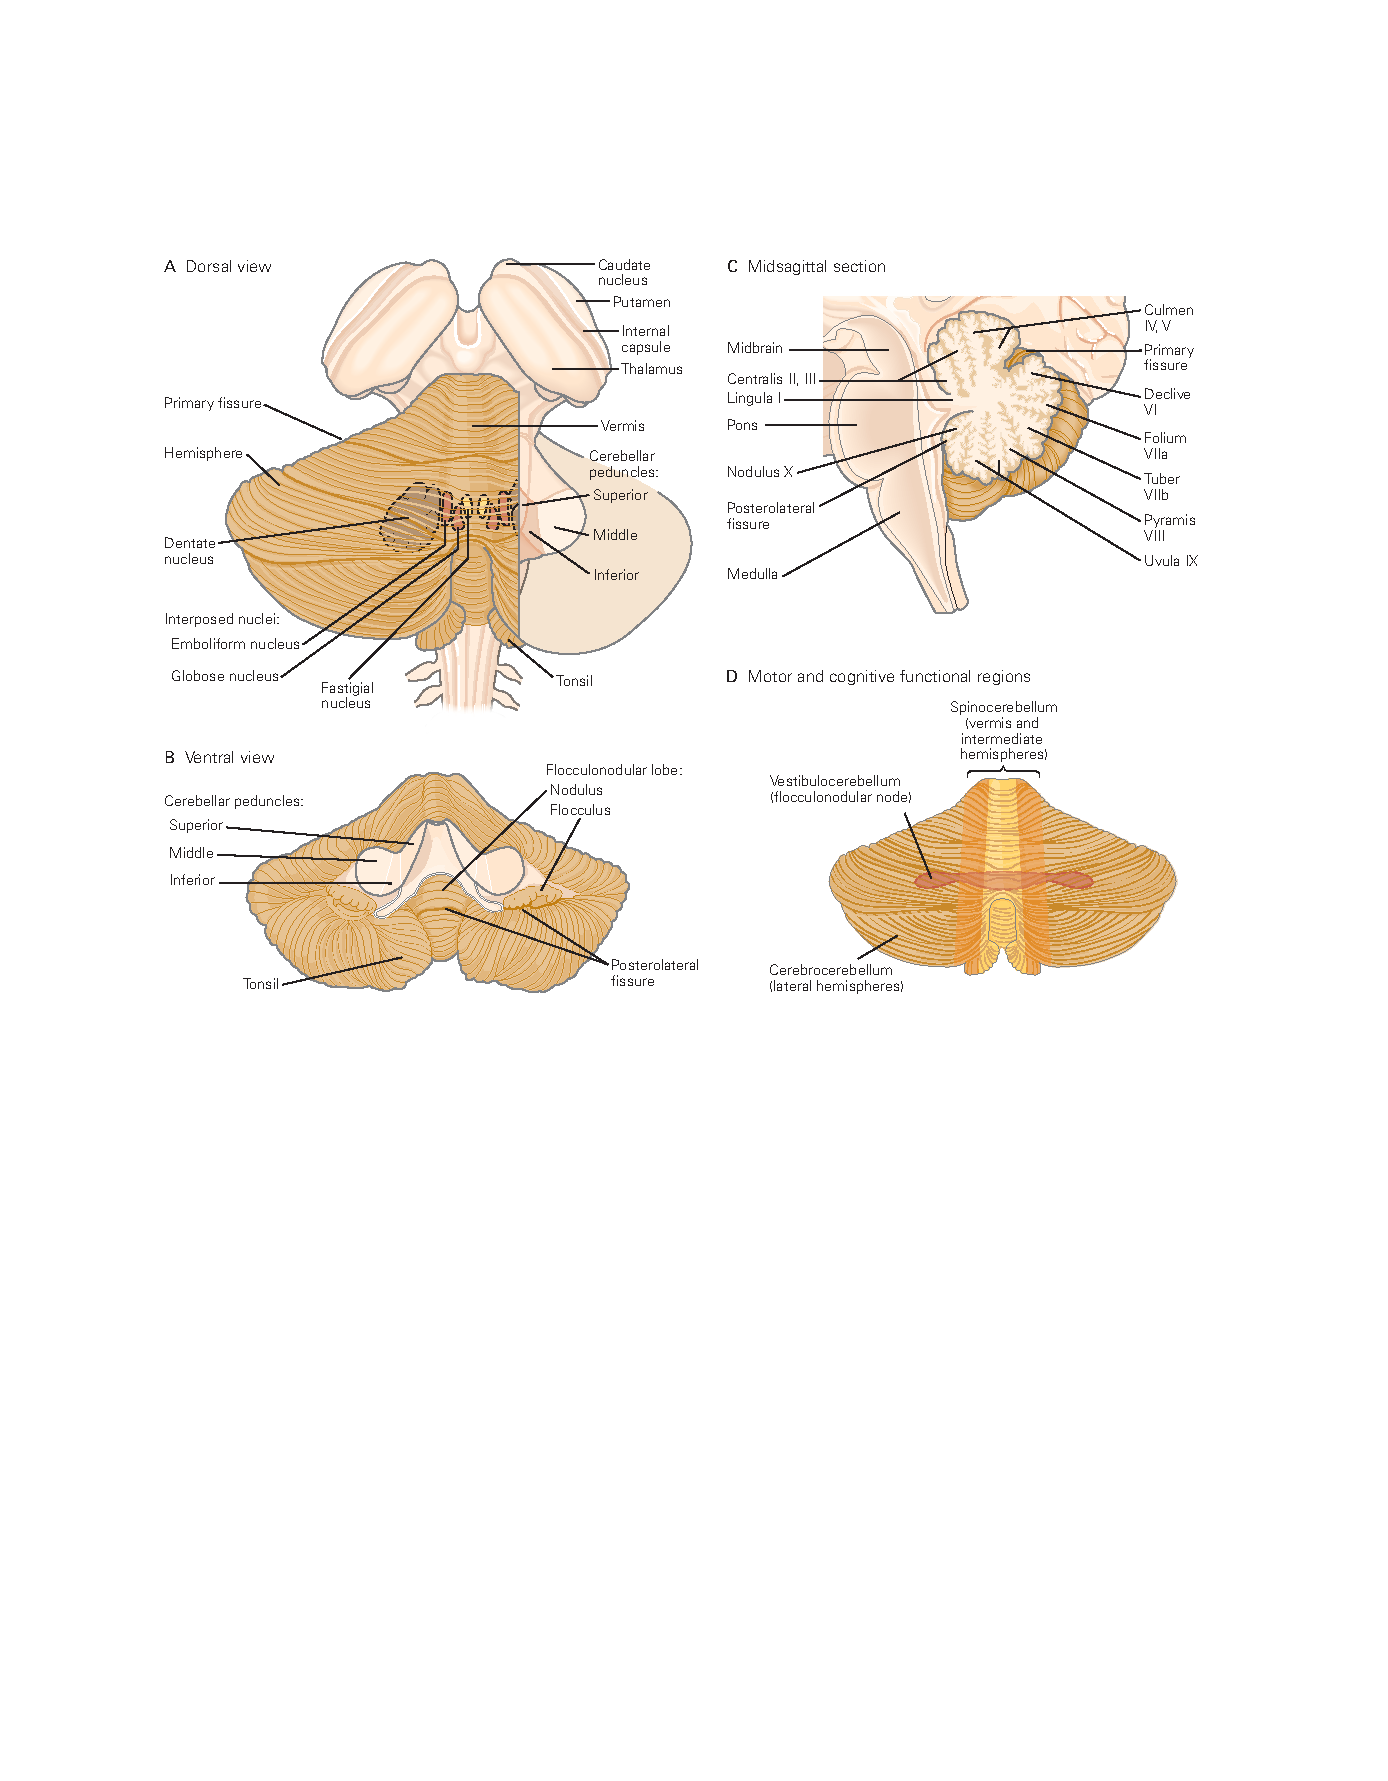
\includegraphics[width=0.9\linewidth]{chap37/fig_37_2}
	\caption{小脑的总体特征\cite{nieuwenhuys2007human}。
		\textbf{A.} 右半球的一部分已被切掉以显示下面的小脑脚。
		\textbf{B.} 小脑显示为与脑干分离。
		\textbf{C.} 通过脑干和小脑的正中矢状切面显示了小脑的分支结构。 
		小脑小叶标有其拉丁名称和拉塞尔的罗马数字名称\cite{larsell1972comparative}。}
	\label{fig:37_2}
\end{figure}



小脑起源于深部核团并通过小脑上脚投射到其他脑区。
主要的例外是絮状结节叶中的一组浦肯野细胞,它们投射到脑干中的前庭核。



\subsection{小脑通过循环回路与大脑皮层相连}

小脑的许多部分与大脑皮层形成循环回路。
大脑皮层通过桥脑核中的中继投射到小脑外侧。
反过来,小脑外侧通过丘脑中的中继投射回大脑皮层。
Peter Strick 和他的同事使用病毒在非人类灵长类动物中进行跨神经元追踪,以表明这种循环回路被组织为一系列平行的闭环,其中小脑的给定部分与大脑皮层的特定部分相互连接(图~\ref{fig:37_3}A)。
通过这些相互联系,小脑与新皮层的广大区域相互作用,包括与运动、前额叶和后顶叶区域的实质性联系。
最近,Strick 的小组还展示了非人类灵长类动物的小脑和基底神经节之间的非突触连接。


使用 1,000 名受试者的\textit{功能性磁共振成像}扫描研究了人类小脑和大脑皮层之间的静息状态连接。
在低频下评估大脑不同区域活动的相关性,通过受试者在休息时的血流量来测量。
他们发现小脑的不同区域在功能上与整个大脑皮层的大脑皮层区域相连(图~\ref{fig:37_3}C)。
总而言之,这些研究表明小脑可能对大脑功能的许多方面产生巨大影响。


\begin{figure}[htbp]
	\centering
	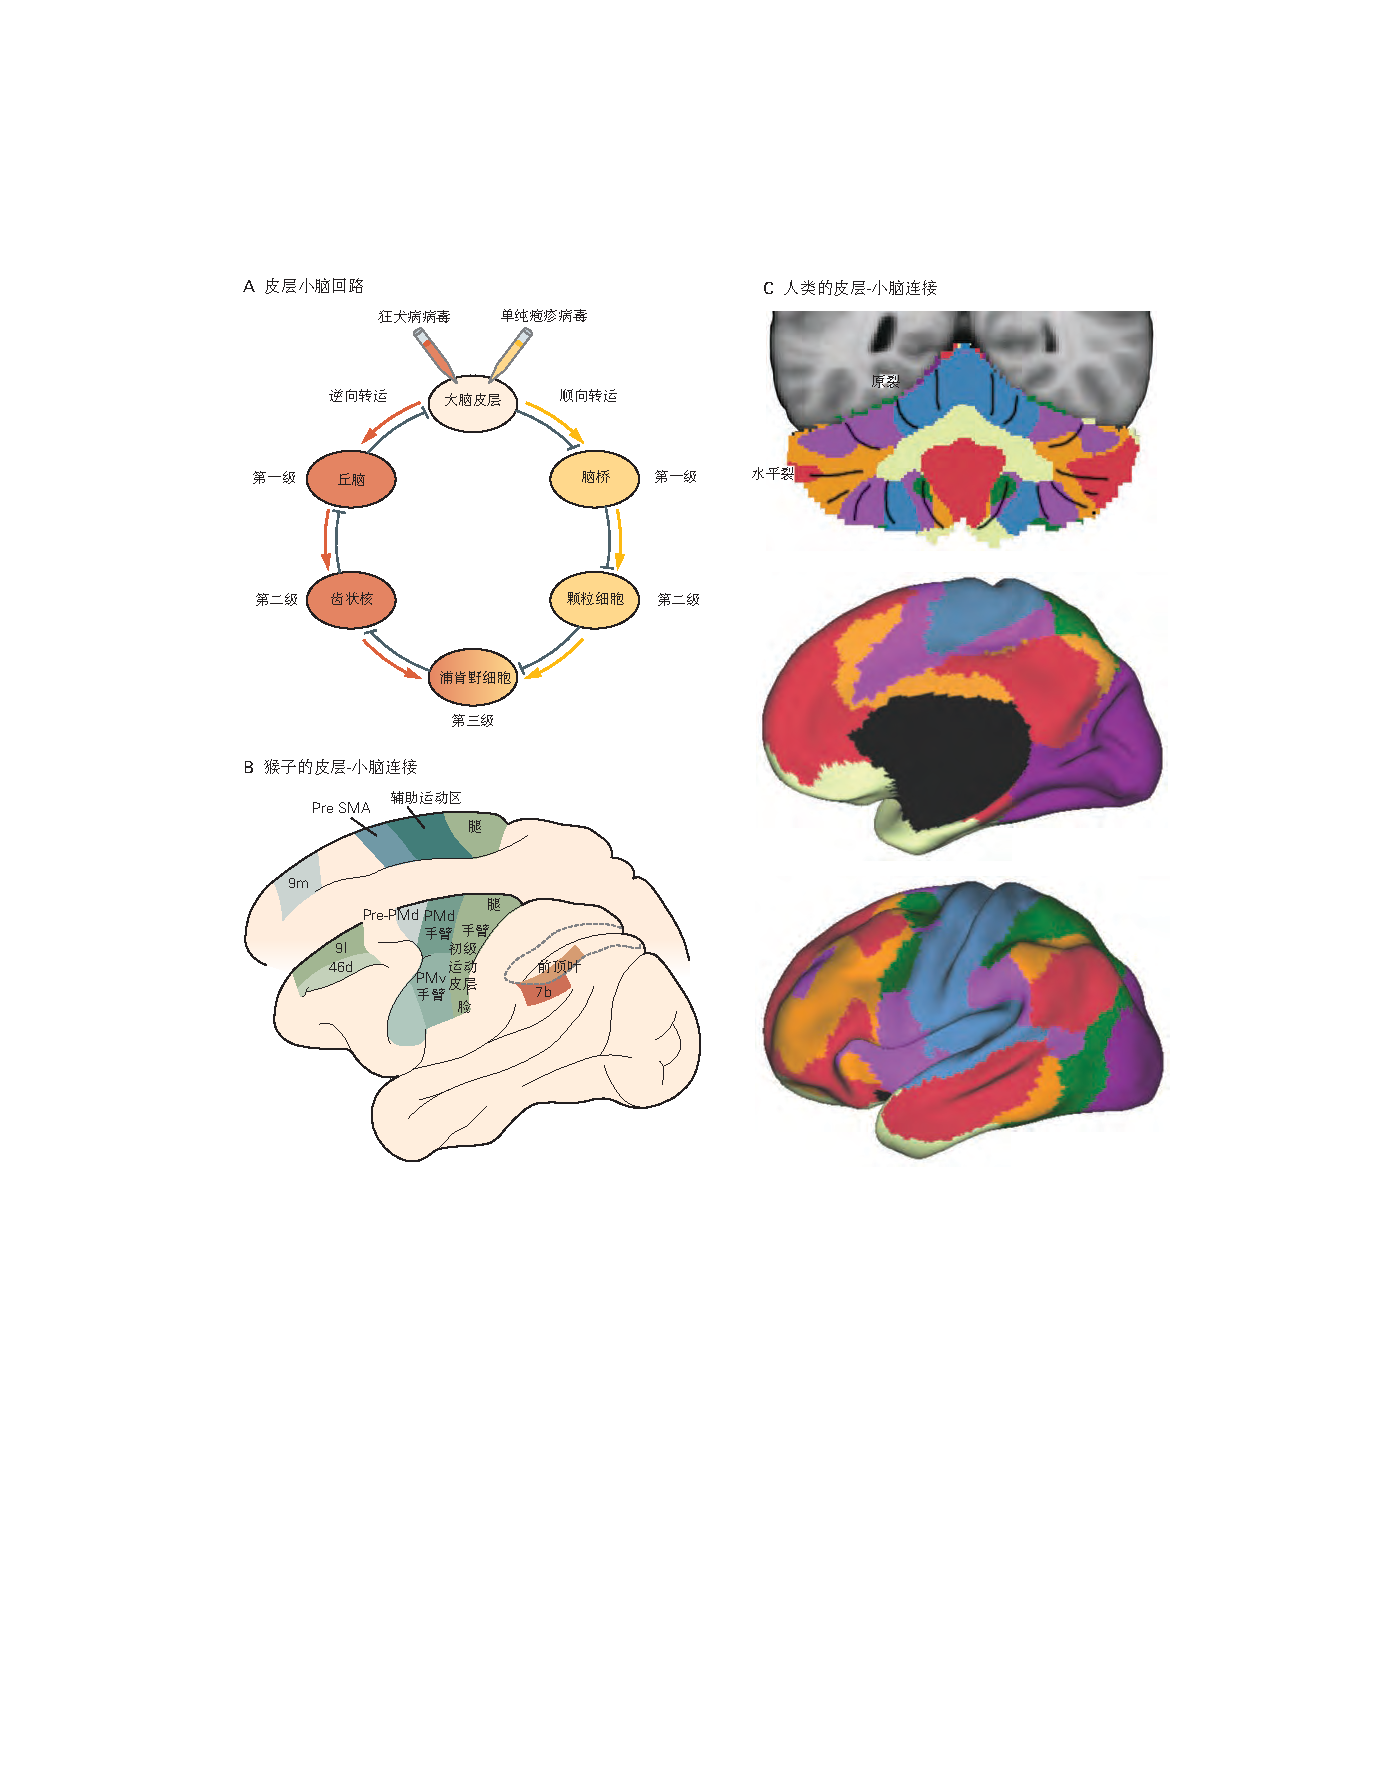
\includegraphics[width=0.9\linewidth]{chap37/fig_37_3}
	\caption{小脑连接到大脑皮层的许多区域\cite{bostan2013cerebellar}。
		\textbf{A.} 用荧光标记的跨突触病毒追踪猴子的皮层小脑回路,这些病毒可以顺行或逆行移动。
		将逆行病毒(如狂犬病病毒)注入大脑皮层,将标记投射到它的神经元,并通过穿过突触,标记通路中的二级和可能更高阶神经元。
		这些在这里以红色显示为一级(丘脑)、二级(深核)和三级神经元(浦肯野细胞)。
		将顺行病毒(例如单纯疱疹病毒)注射到大脑皮层,将标记作为大脑皮层目标的神经元。
		这些在这里以黄色显示为一级(\textit{脑桥})、二级(\textit{颗粒细胞})和三级神经元(\textit{浦肯野细胞})。
		\textbf{B.} 与小脑相连的大脑皮层区域。 数字指的是细胞构造区域。
		(缩写:PMd,背侧前运动皮层;PMv,腹侧前运动皮层)
		\textbf{C.} 人类小脑的彩色编码冠状切面(顶部)和人类大脑皮层的侧视图和内侧视图(底部)从静息中创建 状态功能连接图(基于 1 千名受试者的功能磁共振成像扫描)。
		颜色对应于连接的小脑和大脑区域。
		请注意,小脑在功能上与几乎所有大脑区域相连。}
	\label{fig:37_3}
\end{figure}



\subsection{不同的运动由纵向功能区控制}

小脑可大致分为三个区域,它们在不同类型的运动中具有独特的作用:
前庭小脑、脊髓小脑和小脑(图~\ref{fig:37_4})。


\begin{figure}[htbp]
	\centering
	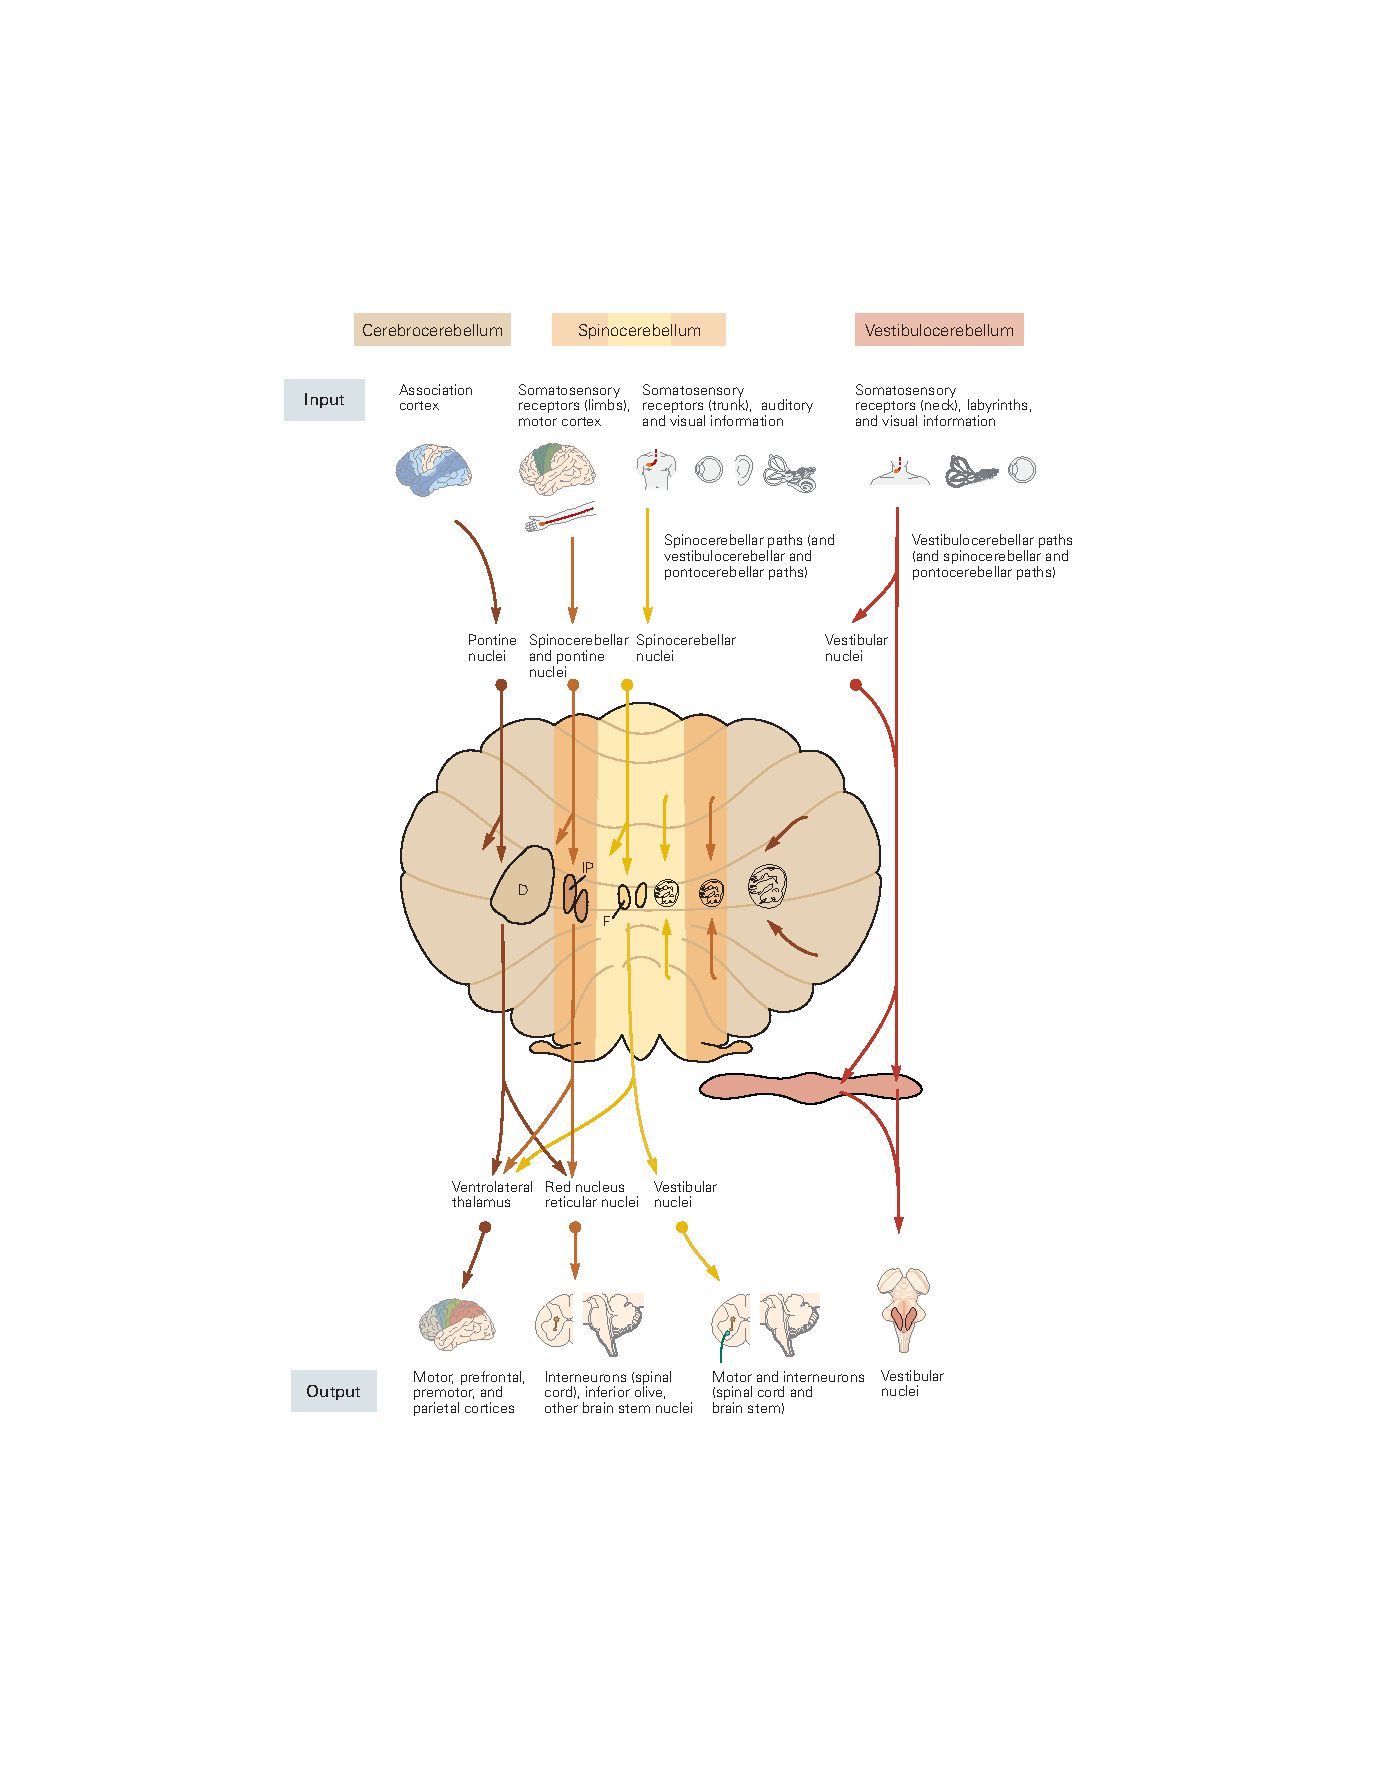
\includegraphics[width=0.7\linewidth]{chap37/fig_37_4}
	\caption{小脑的三个功能区具有不同的输入和不同的输出目标。
		小脑显示为展开状态,箭头表示不同功能区域的输入和输出。
		深核中的身体图基于非人类灵长类动物的解剖追踪和单细胞记录\cite{brooks1981handbook}。}
	\label{fig:37_4}
\end{figure}


前庭小脑由絮状结节叶组成,是小脑最原始的部分。
它接收前庭和视觉输入,投射到脑干中的前庭核团,并参与平衡、其他前庭反射和眼球运动。
它从半规管和耳石器官接收信息,这些器官感知头部的运动及其相对于重力的位置。
大部分前庭输入来自脑干中的前庭神经核。
前庭小脑还接收视觉输入,来自位于上丘下方的中脑深处的前顶核,以及通过脑桥和前顶核的初级和次级视觉皮层。


前庭小脑的独特之处在于其输出绕过小脑深部核团并直接进入脑干中的前庭核团。
前庭小脑中线部分的浦肯野细胞投射到外侧前庭核以调节外侧和内侧前庭脊髓束,后者主要控制轴向肌肉和肢体伸肌以确保站立和步态期间的平衡(图~\ref{fig:37_5}A)。
通过病变或疾病破坏这些投射会损害平衡。


\begin{figure}[htbp]
	\centering
	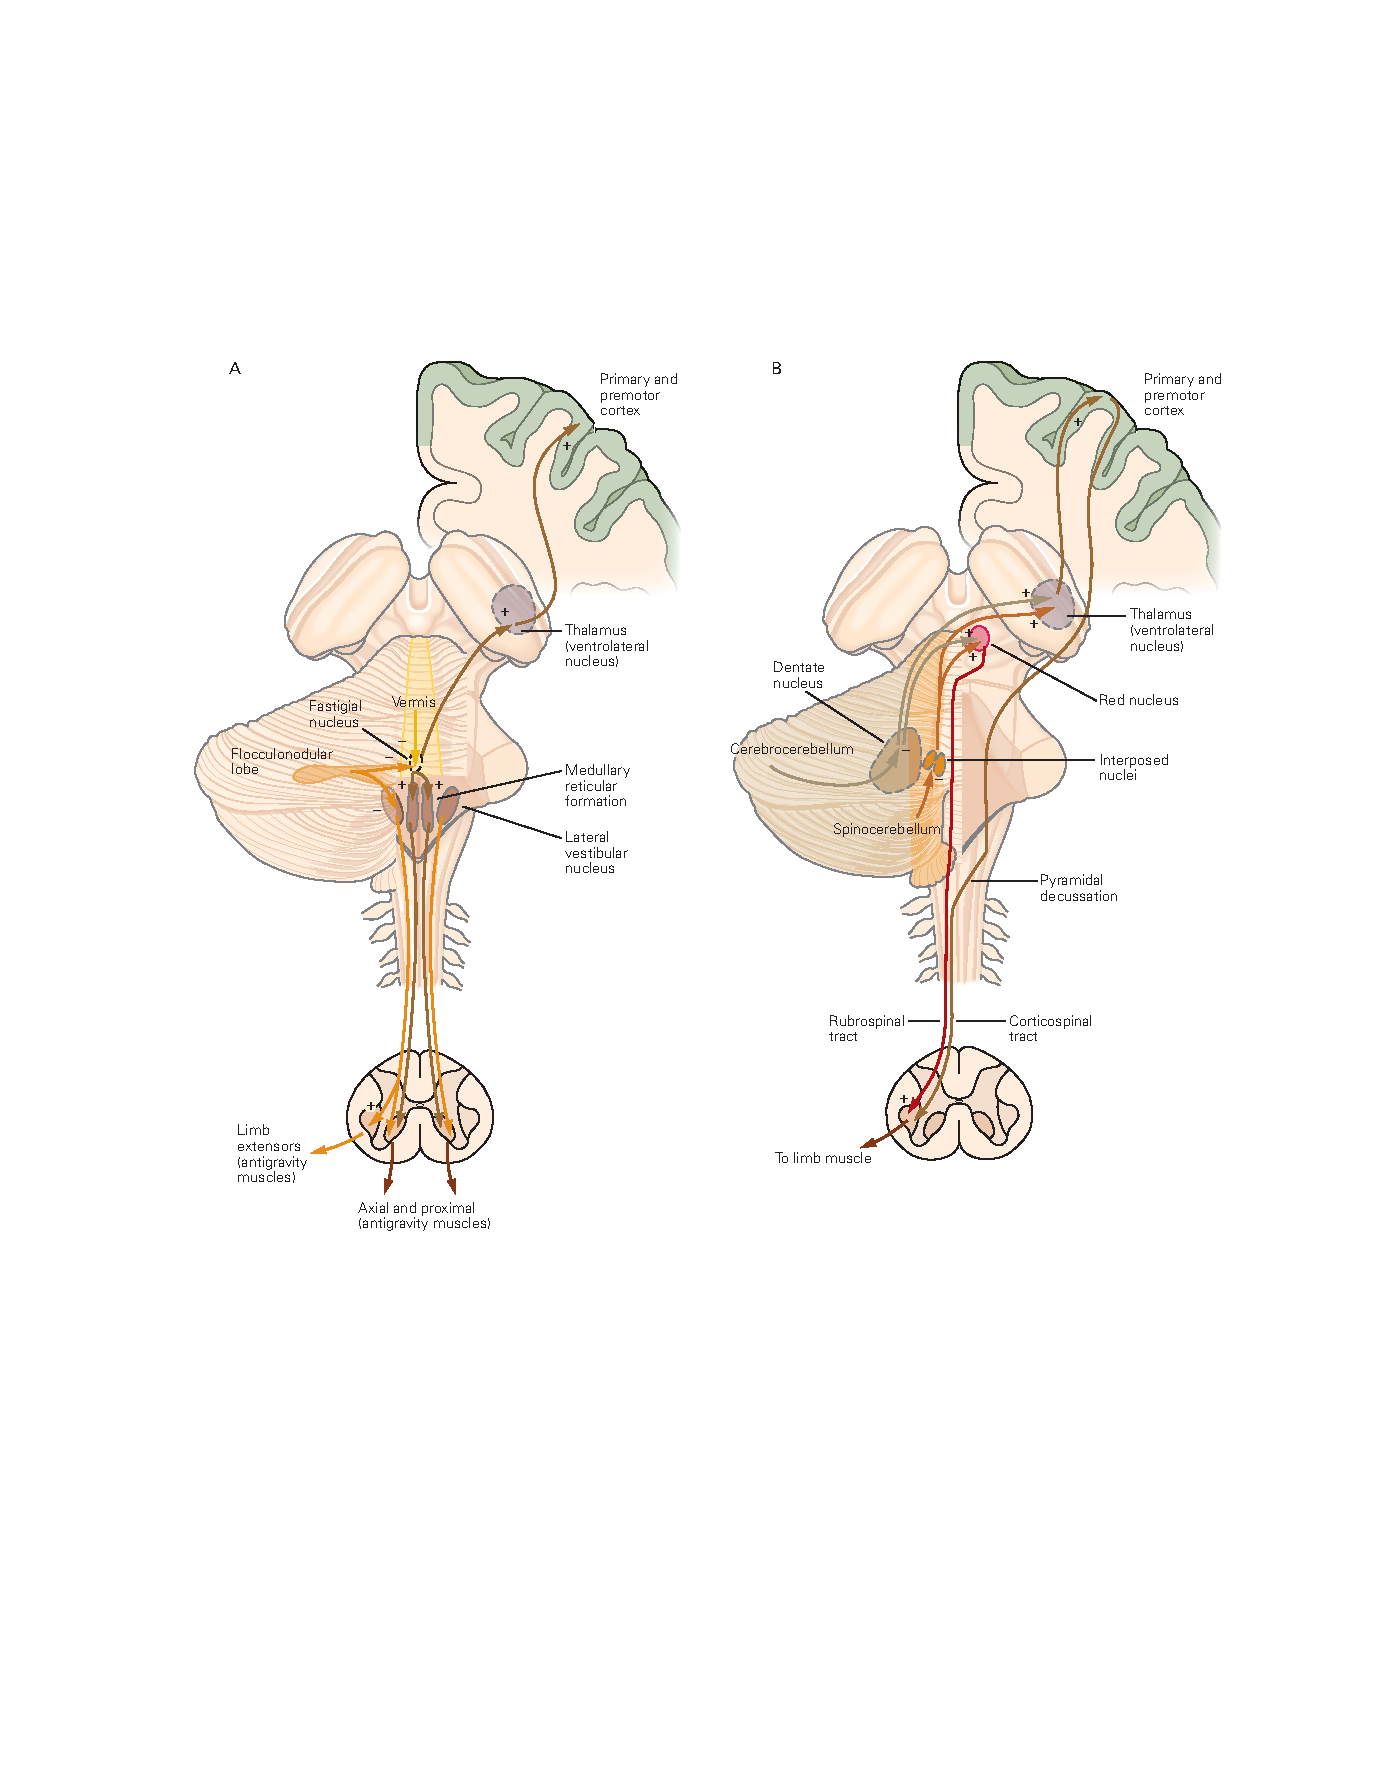
\includegraphics[width=0.9\linewidth]{chap37/fig_37_5}
	\caption{小脑的输入和输出通路。
		\textbf{A.} 前庭小脑和小脑蚓体中的核团控制近端肌肉和\textit{肢体伸肌}。
		前庭小脑(絮状结节叶)接收来自前庭迷路的输入并直接投射到前庭核团。
		\textit{小脑蚓体}接收来自颈部和躯干、前庭迷路以及视网膜和眼外肌的输入。
		它的输出集中在脑干的腹内侧下行系统,主要是网状脊髓束和前庭脊髓束以及作用于内侧运动神经元的皮质脊髓纤维。
		为清楚起见,省略了前庭神经核的动眼神经连接。
		\textbf{B.} 小脑半球中间和外侧部分的核团控制肢体和轴向肌肉。
		每个半球的中间部分(脊髓小脑)接收来自四肢的感觉信息并控制作用于同侧肢体的背外侧下行系统(红核脊髓束和皮层脊髓束)。
		每个半球的外侧区域(小脑)通过桥脑核接受皮层输入,并通过丘脑腹外侧核影响运动和前运动皮层,并直接影响红核。}
	\label{fig:37_5}
\end{figure}


外侧前庭小脑损伤后最显着的缺陷是向损伤侧的平滑跟随眼球运动。
患有左侧前庭小脑损伤的患者可以平稳地跟踪向右移动的目标,但只能很差地跟踪向左运动,主要使用扫视(图~\ref{fig:37_6}A)。
这些患者可以对头部旋转有正常的前庭眼反射反应,但不能通过固定随头部旋转的物体来抑制反射(图~\ref{fig:37_6}B)。
如果外侧前庭小脑被听神经瘤压迫,这些缺陷通常会发生,听神经瘤是一种生长在第八脑神经上的良性肿瘤,因为它直接走行在外侧前庭小脑下方。


\begin{figure}[htbp]
	\centering
	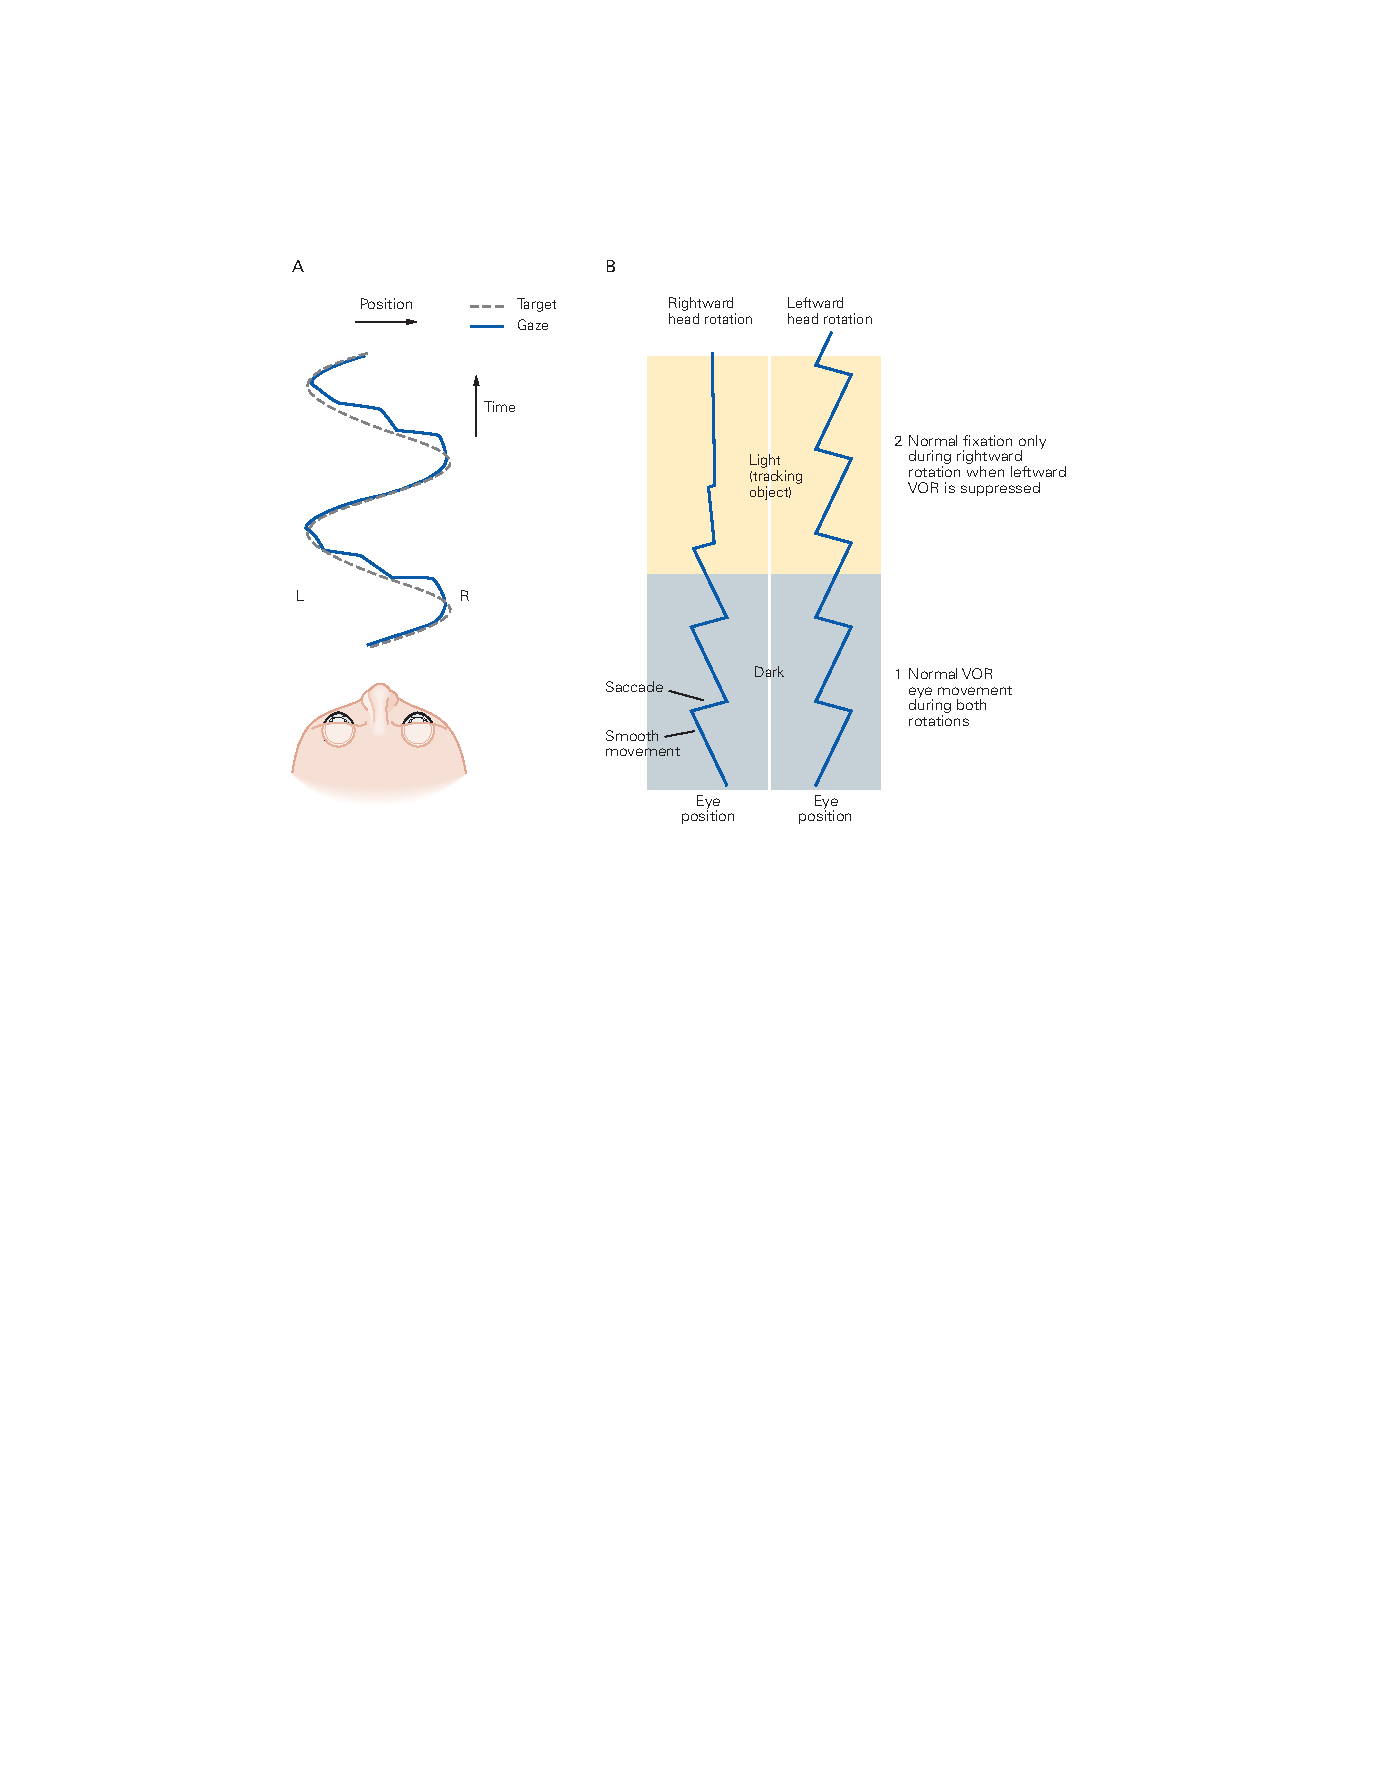
\includegraphics[width=0.8\linewidth]{chap37/fig_37_6}
	\caption{前庭小脑的病变对平滑跟随眼球运动有很大影响。
		\textbf{A.} 当目标从左移动到右时,正弦曲线目标运动通过平滑跟随眼球运动进行跟随。
		由于左侧前庭小脑的损伤,当目标从右向左移动时,平稳跟随会被扫视打断。
		\textbf{B.} 在同一名患者中,对前庭刺激的反应是正常的,而在向左旋转期间物体固定被打乱。
		左侧和右侧的痕迹显示了在不同的会话中经历的向右和向左的头部旋转引起的眼球运动。
		在每次治疗中,患者坐在一张不断向一个方向旋转的椅子上,先是在黑暗中,然后是在光线中,同时注视着一个与他一起移动的目标。
		(1) 在黑暗中,眼睛在两个方向的旋转过程中表现出正常的\textit{前庭眼反射}:眼睛在与头部旋转相反的方向上平稳移动,然后在头部旋转的方向上以扫视复位。
		(2) 光照下,头向右转时眼位正常:对目标的注视良好,前庭眼反射受到抑制。
		然而,在向左头部旋转期间,受试者无法注视物体并且无法抑制前庭眼反射。}
	\label{fig:37_6}
\end{figure}


脊髓小脑由小脑半球的\textit{小脑蚓体}和中间部分组成(图~\ref{fig:37_4})。
它之所以如此命名,是因为它通过背侧和腹侧脊髓小脑束接收来自脊髓的广泛输入。
这些通路传递有关触摸、压力和肢体位置以及脊髓中间神经元尖峰活动的信息。
因此,这些输入为小脑提供了有关生物体及其环境不断变化的状态的各种信息。


\textit{小脑蚓体}接收来自头部和身体近端部分的视觉、听觉和前庭输入以及躯体感觉输入。
它通过顶核投射到皮层和脑干区域,从而产生控制身体和四肢近端肌肉的内侧降系统(图~\ref{fig:37_5}A)。
\textit{小脑蚓体}控制姿势和运动以及眼球运动。
例如,\textit{小脑蚓体}动眼神经区的病变会导致眼球扫视运动超过目标,就像小脑损伤患者的手臂运动超过目标一样。


半球的相邻中间部分也接收来自四肢的体感输入。
这里的神经元投射到中间核,后者为大脑对侧的外侧皮层脊髓和红核脊髓系统提供输入,并控制四肢和手指的更远端肌肉(图~\ref{fig:37_5}B)。
由于皮层脊髓和红核脊髓系统在下行至脊髓时穿过中线,因此小脑病变会扰乱同侧肢体运动。


小脑包括半球的外侧部分(图~\ref{fig:37_4})。
这些区域在系统发育上是最近的,并且相对于人类和猿类小脑的其余部分比猴子和猫大得多。
该区域的几乎所有输入和输出都涉及与大脑皮层的连接。
输出通过齿状核传输,齿状核通过丘脑投射到对侧运动、前运动、顶叶和前额皮层。
齿状核也投射到对侧红核。
侧半球有很多功能,但似乎最广泛地参与了运动的规划和执行。
它们还在与运动规划无关的认知功能中发挥作用,例如视觉空间和语言过程。
现在有一些相关证据表明小脑半球与精神分裂症(第 ~\ref{chap:chap60}~章)、肌张力障碍(第~\ref{chap:chap38}~章)和孤独症(第~\ref{chap:chap62}~章)等方面有关。


小脑功能的两个重要原则已经从小脑皮层和小脑深部核团中单个神经元在手臂运动过程中的动作电位的记录中出现,以及特定小脑区域的受控的暂时失活。


首先,这些区域的神经元与随意运动有关,会剧烈激活。
小脑输出量与运动的方向和速度有关。
深核被组织成不同肢体和关节的体位图,就像在运动皮层中一样,尽管小脑皮层的组织被描述为具有多个断开和部分图的“断裂体位图”。
此外,小脑神经元放电调制开始与运动之间的间隔与运动皮层神经元的间隔非常相似。
这一结果强调了小脑参与了与大脑皮层同步运作的循环回路。


其次,小脑提供肌肉收缩的前馈控制以调节运动的时间。
小脑输出不是等待感觉反馈,而是预测将运动平稳、准确、快速地带到其期望终点所需的肌肉收缩。
这些机制的失败会导致小脑疾病的意向性震颤。
例如,快速的单关节运动由主动肌的收缩启动,并由拮抗肌适时的收缩终止。
拮抗剂的收缩在运动的早期就开始了,远早于感觉反馈到达大脑的时间,因此必须作为运动的一部分进行编程。
然而,当齿状核和插入核在实验上失活时,拮抗肌的收缩会延迟,直到肢体超过其目标。
正常运动中拮抗剂的程序化预期收缩被感官反馈驱动的校正所取代。
这种校正本身是不对称的,会导致另一个错误,需要进行新的调整(图~\ref{fig:37_7})。


\begin{figure}[htbp]
	\centering
	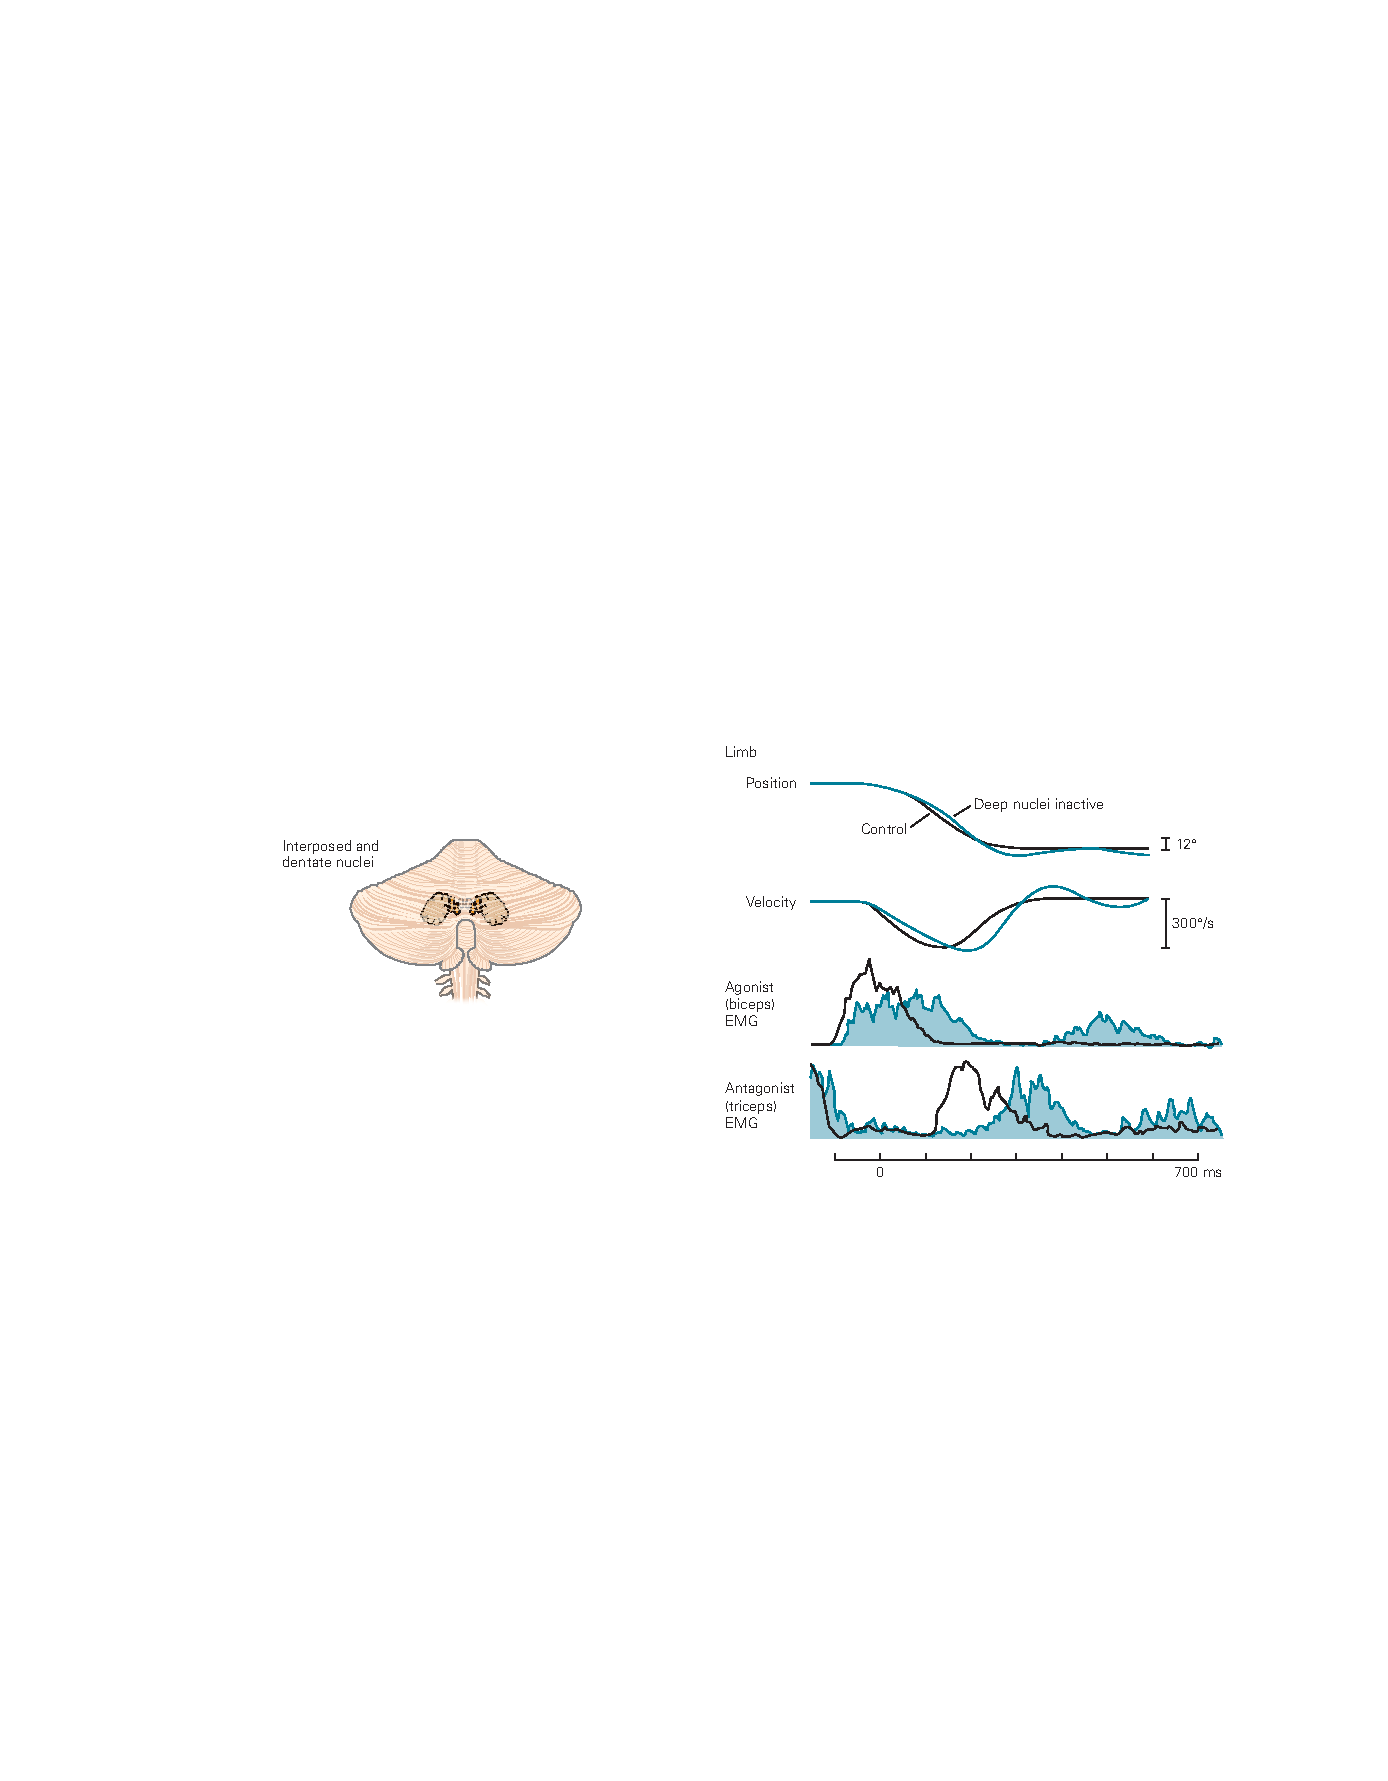
\includegraphics[width=0.75\linewidth]{chap37/fig_37_7}
	\caption{插入和齿状核参与快速运动期间激动剂和拮抗剂激活的精确时间。
		插入的(内侧)和齿状(外侧)核在小脑的绘图中突出显示。肢体运动的记录显示了猴子通常如何进行快速的肘部屈曲肢体运动,并在中间和齿状核因冷却而失活时尝试进行相同的运动。
		\textit{肌电图}迹线显示肢体位置和速度以及二头肌和三头肌的 \textit{肌电图} 反应。
		当深部核失活时,\textit{主动肌}(二头肌)的激活变得更慢且持续时间更长。
		在正确位置停止运动所需的\textit{拮抗肌}(三头肌)的激活同样被延迟和延长,因此初始运动超过其适当的范围。
		运动连续阶段的延迟会产生类似于小脑损伤患者所见的终末震颤的振荡。}
	\label{fig:37_7}
\end{figure}



\section{小脑皮层由具有相同基本微回路的重复功能单元组成}

小脑皮层微回路的细胞组织是惊人的,小脑研究的前提之一是微回路的细节是小脑如何工作的重要线索。
在本节中,我们将描述微回路的三个主要特征。



\subsection{小脑皮层分为三个功能专门层}

小脑皮层的三层包含不同种类的神经元,并且在功能上是专门的(图~\ref{fig:37_8})。


\begin{figure}[htbp]
	\centering
	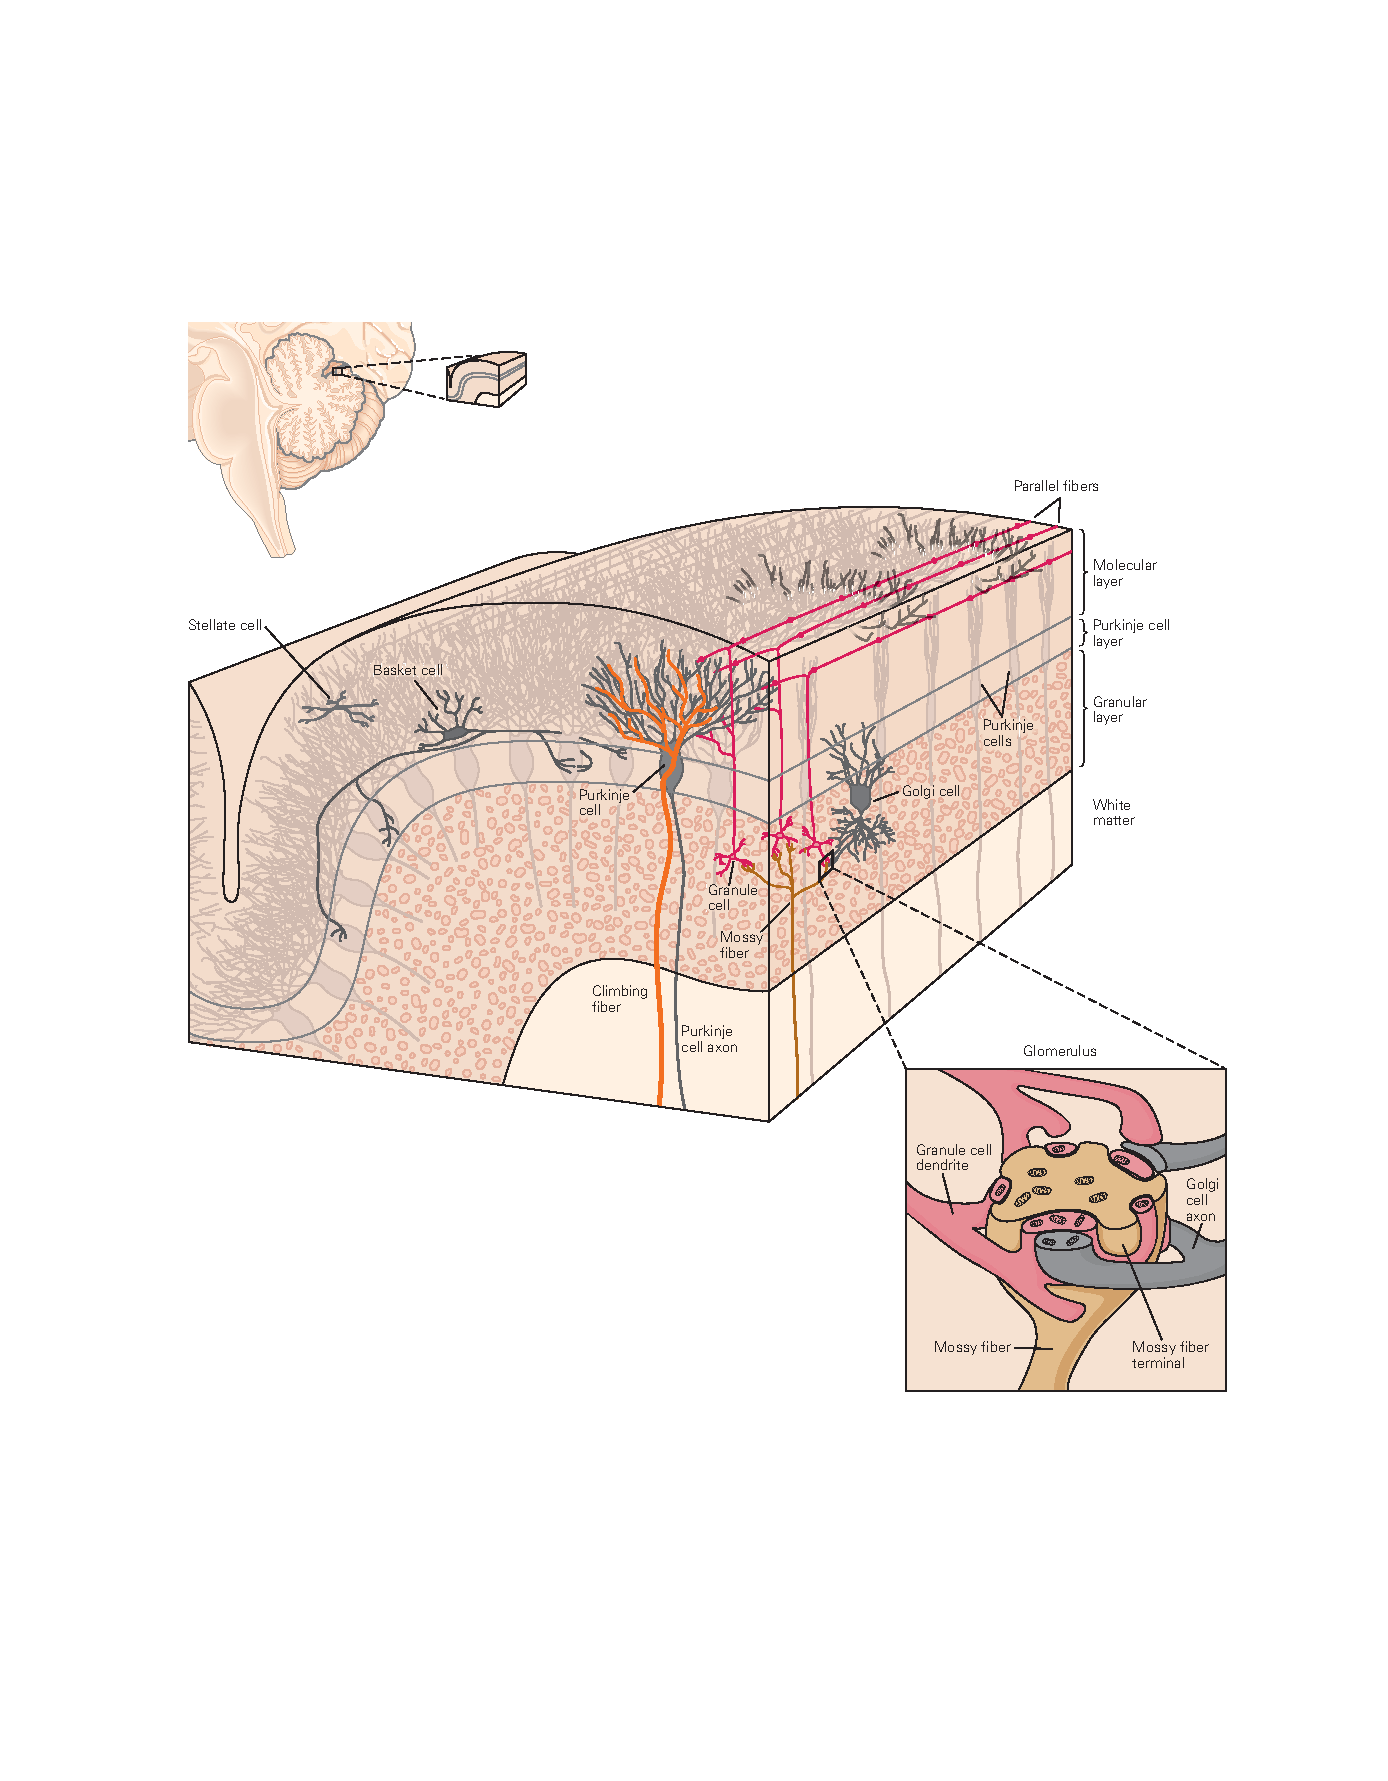
\includegraphics[width=0.9\linewidth]{chap37/fig_37_8}
	\caption{小脑皮层包含五种主要类型的神经元,分为三层。
		单个小脑叶的垂直剖面说明了小脑皮层的一般组织。
		还显示了颗粒层中小脑肾小球的细节。
		肾小球是由苔藓纤维的球状轴突末端和几个高尔基体和颗粒细胞的树突形成的突触复合体。
		线粒体存在于\textit{小脑小球}的所有结构中,与其高代谢活性一致。}
	\label{fig:37_8}
\end{figure}


最深的或粒度层是输入层。
它包含大量颗粒细胞,估计有 1 千亿个,它们在组织学切片中显示为小的、密集的、深色染色的细胞核。
颗粒层还包含一些较大的高尔基体细胞,在一些小脑区域,还包含少量其他神经元,例如\textit{卢加洛细胞}、单极刷状细胞和吊灯细胞。
苔藓纤维是小脑的两个主要传入输入之一,终止于这一层。
苔藓纤维的球根状末端刺激称为小脑肾小球的突触复合体中的颗粒细胞和高尔基神经元(图~\ref{fig:37_8})。
正如我们稍后在讨论小脑中的循环回路时将看到的那样,高尔基细胞会抑制颗粒细胞。


中间层或浦肯野细胞层是小脑皮层的输出层。
该层由单片浦肯野细胞体组成,每个直径为 50 至 80 微米。
浦肯野细胞的扇形树突树向上延伸到分子层,在那里它们接收来自小脑的第二种主要传入神经、攀爬纤维以及颗粒细胞和抑制性中间神经元的输入。
浦肯野细胞轴突传导小脑皮层的全部输出,投射到下方白质的深核或脑干的前庭核,在那里它们释放抑制性递质\textit{$ \gamma $-氨基丁酸}。


最外层或分子层包含浦肯野细胞的空间极化树突,其在前后方向延伸约 1 至 3 毫米,但在内外方向仅占据非常狭窄的区域。
分子层包含两种类型的“分子层中间神经元”星状细胞和篮状细胞的细胞体和树突,它们都抑制浦肯野细胞。
它还包含颗粒细胞的轴突,称为平行纤维,因为它们平行于叶片的长轴延伸(图~\ref{fig:37_8})。
平行纤维垂直于浦肯野细胞的树突树延伸,因此有可能与大量浦肯野细胞中的每一个形成一些突触。



\subsection{攀缘纤维和苔藓纤维传入系统编码和处理信息的方式不同}

小脑中的两种主要传入纤维,苔藓纤维和攀缘纤维,可能介导不同的功能。
两者都与小脑深部核团和小脑皮层中的神经元形成兴奋性突触。
然而,它们终止于小脑皮层的不同层,通过非常不同的突触会聚和发散模式影响浦肯野细胞,并在浦肯野细胞中产生不同的电事件。


攀爬纤维起源于脑干的下橄榄核,将周围和大脑皮层的感觉信息传递给小脑。
攀缘纤维之所以如此命名,是因为每根纤维都像树上的藤蔓一样缠绕在浦肯野神经元的近端树突上,形成无数的突触接触(图~\ref{fig:37_9})。
每个浦肯野神经元仅接收来自单个攀爬纤维的突触输入,但每个攀爬纤维接触 1 到 10 个浦肯野细胞,这些细胞沿着小脑皮层的旁矢状带按地形排列。
实际上,来自相关橄榄神经元簇的轴突终止于横跨数个叶状叶的薄的矢状旁带,而来自一条带的浦肯野细胞汇聚在深核中的一组共同神经元上。


\begin{figure}[htbp]
	\centering
	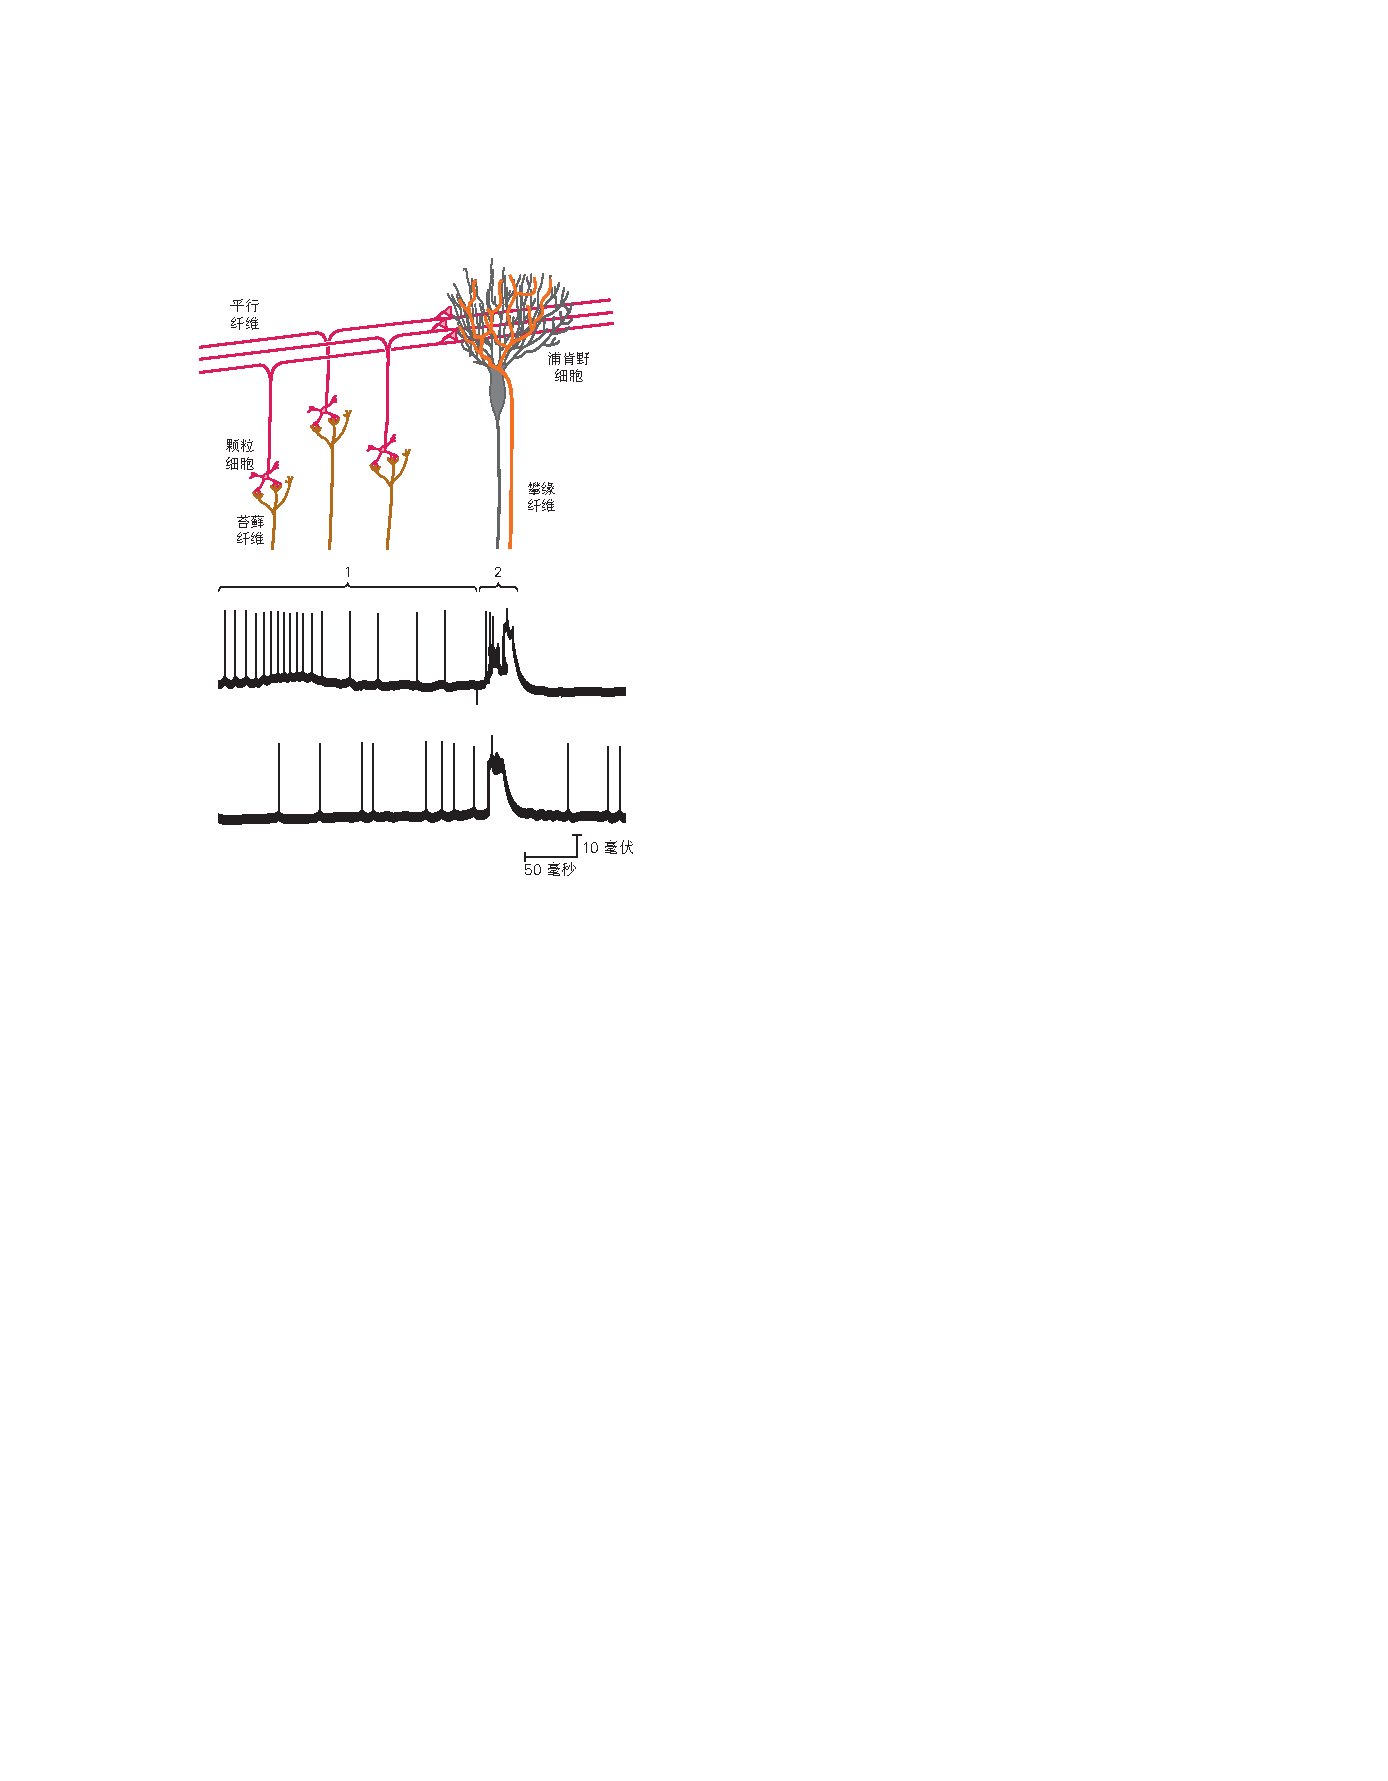
\includegraphics[width=0.45\linewidth]{chap37/fig_37_9}
	\caption{从小脑浦肯野细胞在细胞内记录的简单和复杂的尖峰信号。
		简单的尖峰由苔藓纤维输入 (1) 产生,而复杂的尖峰由攀缘纤维突触 (2) 诱发\cite{martinez1971electrogenesis}。}
	\label{fig:37_9}
\end{figure}


攀缘纤维对浦肯野细胞的电活动具有异常强大的影响。
攀缘纤维中的每个动作电位都会在突触后浦肯野细胞的体细胞和树突中产生延长的电压门控 \ce{Ca^2+} 电导。
这会导致长时间的去极化,从而产生称为“复杂尖峰”的电事件:
一个初始的大幅值动作电位,然后是一个高频爆发的较小幅值动作电位(图~\ref{fig:37_9})。
这些较小的尖峰是否沿着浦肯野细胞的轴突向下传递尚不清楚。
在清醒的动物中,复杂的尖峰信号以低速率自发出现,通常约为每秒一个。
特定的感觉或运动事件会导致在与这些事件相关的精确时间发生一两个复杂的峰值。


苔藓纤维起源于脊髓和脑干中的细胞体。
它们携带来自外周的感觉信息以及通过桥脑核从大脑皮层报告当前运动命令(第~\ref{chap:chap30}~章)的感觉信息和必然放电。
苔藓纤维通过具有有趣的收敛和发散模式的多突触通路影响浦肯野细胞。
单个苔藓纤维通过颗粒细胞和平行纤维起作用,对浦肯野细胞的输出影响很小,但总的来说,整个苔藓纤维群对小脑输出有巨大影响。


苔藓纤维在颗粒层的颗粒细胞树突上形成兴奋性突触(图 ~\ref{fig:37_8})。
每个颗粒细胞有三到五个短树突,每个树突都与一根苔藓纤维接触。
由于缺乏输入,颗粒细胞对其不同苔藓纤维突触的空间整合并不广泛;
然而,细胞可能是来自多种感觉方式和运动必然放电的苔藓纤维的汇聚点。
下一个突触中继位于颗粒细胞轴突和浦肯野细胞之间,以非常广泛的发散和收敛分布信息。
平行纤维允许每个苔藓纤维影响大量浦肯野细胞,每个浦肯野细胞可能与来自 200,000 到 100 万个颗粒细胞之间某处的轴突接触。
重要的是,为了响应不断变化的条件,平行纤维和浦肯野细胞之间的突触处的小脑输出似乎具有巨大的适应潜力。
似乎在任何给定时间,这些突触中只有一小部分处于活动状态。


平行纤维在浦肯野细胞中产生短暂、小的兴奋性电位(图~\ref{fig:37_9})。
这些电位汇聚在细胞体中并扩散到轴突的初始部分,在那里它们产生称为“简单尖峰”的常规动作电位,沿着轴突传播。
在清醒的动物中,浦肯野细胞发出稳定的简单尖峰流,即使动物安静地坐着,自发放电率也高达每秒 100 次。
在眼睛、手臂和面部活动期间,浦肯野细胞以高达每秒数百个脉冲的速率放电。


攀缘纤维和苔藓纤维/平行纤维系统似乎专门用于传输不同种类的信息。
攀爬纤维会导致复杂的尖峰,似乎专门用于事件检测。
虽然复杂的尖峰很少出现,但多条攀爬纤维的同步发射使它们能够发出重要事件的信号。
同步性的出现部分是因为下橄榄核中许多神经元之间的信号以电张力方式发生(在间隙连接通道)。
相比之下,浦肯野细胞中简单尖峰的高放电率可以通过苔藓纤维输入以分级方式向上或向下调制,从而编码外周刺激或中央产生的行为的幅度和持续时间。



\subsection{小脑微回路架构建议进行规范计算}

小脑微回路在小脑皮层表面被复制多次。
这种重复的结构和收敛和发散模式导致了这样的建议,即由于每个这样的模块都有相同的结构和收敛和发散模式,小脑皮层对其所有输入执行相同的基本“规范”计算,并且它 可能以类似的方式为所有小脑输出系统转换小脑输入。
检查小脑微回路图(图~\ref{fig:37_10})揭示了许多不同的计算组件。
一个普遍特征是浦肯野细胞或小脑深部核团存在平行的兴奋性和抑制性通路。 另一个一般特征是循环循环的普遍存在。


\begin{figure}[htbp]
	\centering
	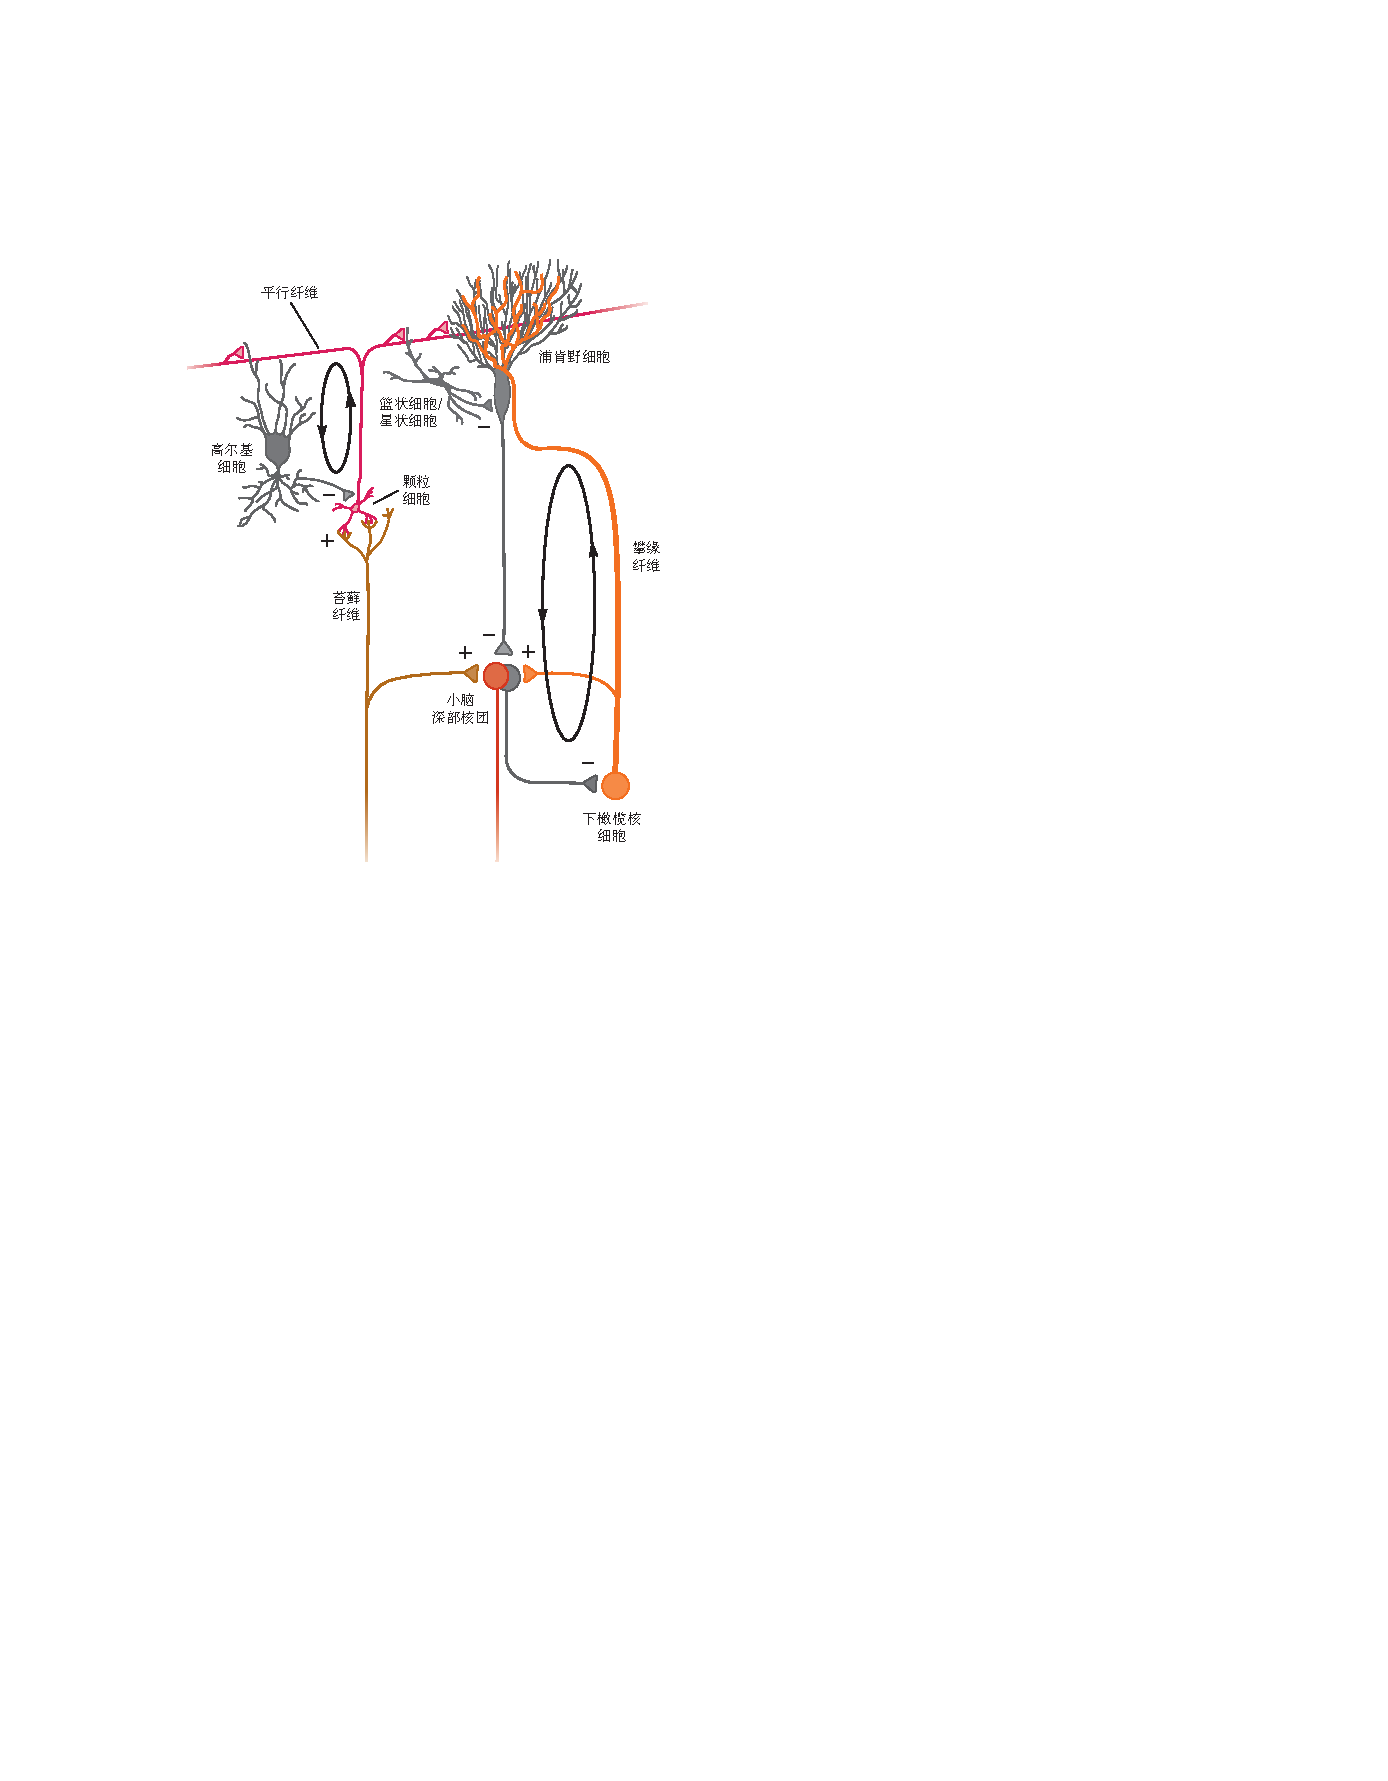
\includegraphics[width=0.5\linewidth]{chap37/fig_37_10}
	\caption{小脑微电路的突触组织。
		兴奋和抑制在小脑皮层和深核中汇聚。
		循环回路涉及小脑皮层内的高尔基细胞和小脑外的下橄榄\cite{raymond1996cerebellum}。}
	\label{fig:37_10}
\end{figure}


从苔藓纤维传递到颗粒细胞再到浦肯野细胞的兴奋性输入与通过两个分子层中间神经元、星状细胞和篮状细胞的前馈抑制性输入并行工作。
这两个中间神经元都接收来自平行纤维的输入并抑制浦肯野细胞,但它们具有完全不同的结构。


星状细胞的短轴突与附近的浦肯野细胞树突接触。
因此,星状细胞在局部起作用,因为它和它抑制的浦肯野细胞被相同的平行纤维激发。
相比之下,篮式细胞的作用更为广泛。 它的轴突垂直于平行纤维(图~\ref{fig:37_8})并在浦肯野细胞上产生侧翼抑制,浦肯野细胞从平行纤维而不是那些激发篮子细胞的纤维接收输入。
星状细胞通过位于远端树突上的突触影响浦肯野细胞,而篮状细胞在浦肯野细胞的细胞体上形成强大的突触,并且似乎被定位为对浦肯野细胞的简单尖峰产生强大的影响。
值得注意的是,即使在小脑微回路结构被描述 60 年后,分子层中间神经元的功能作用仍然是个谜。


兴奋性和抑制性通路的汇聚也是小脑深部核团的一个主要特征。
在这里,来自浦肯野细胞的抑制性输入与来自苔藓和攀缘纤维的轴突侧枝的兴奋性输入汇合(图~\ref{fig:37_10})。
因此,苔藓纤维以两种方式影响深核中的目标神经元:直接通过兴奋性突触和间接通过小脑皮层和抑制性浦肯野细胞的通路。
即使没有突触输入,小脑深部核团的神经元也会自发活跃,因此浦肯野细胞的抑制性输出既调节这种内在活动,又塑造从苔藓纤维传输到深部核团的兴奋信号。
在小脑的几乎所有部分,从攀行纤维到小脑深部核团的侧支为兴奋性和抑制性输入的类似相互作用创造了机会。



循环循环

一个重要的循环回路完全包含在小脑皮层内,并使用高尔基细胞来塑造颗粒细胞的活动,即小脑皮层中的输入元件。
高尔基细胞从苔藓纤维接收一些大的兴奋性输入,从平行纤维接收许多较小的兴奋性输入,并从邻近的高尔基细胞接收抑制性输入。
来自高尔基细胞的 GABAergic 末端抑制颗粒细胞(图 ~\ref{fig:37_10}),从而调节颗粒细胞的活性和平行纤维传递的信号。
这个循环是重要处理可能发生在颗粒层内的证据。
它可能会缩短颗粒细胞爆发的持续时间,限制颗粒细胞对其苔藓纤维输入的兴奋性反应的幅度,或者可以确保颗粒细胞仅在一定数量的苔藓纤维输入处于活动状态时才会做出反应。


第二个循环回路为浦肯野细胞提供了一种调节自身攀爬纤维输入的方法(图~\ref{fig:37_10})。
浦肯野细胞抑制投射到下橄榄的小脑深核中的 $\gamma$-氨基丁酸 能抑制性神经元。
当一组浦肯野细胞的单峰发放减少时,这些抑制性中间神经元的活动增加,导致下橄榄中神经元的兴奋性降低。
下橄榄的兴奋性降低既降低了投射到原始浦肯野细胞群的攀爬纤维动作电位的概率,也降低了攀爬纤维动作电位每次爆发的持续时间。
在关于小脑学习的部分,我们将看到这个循环回路如何让小脑皮层控制输入,从而导致其浦肯野细胞突触发生适应性变化。



\section{假设小脑执行几种一般计算功能}

我们知道小脑对于运动控制和一些非运动功能很重要。
尽管我们还不知道小脑回路如何控制这些功能,但我们能够确定似乎特别“小脑”的控制方面。
这些包括可靠的前馈控制、内部定时控制、感官输入与必然放电的集成,以及通过内部模型进行的状态估计。



\subsection{小脑有助于前馈感觉运动控制}

感官反馈本质上是延迟的。
因此,当运动开始时,在接收到关于该运动的任何有用的感官反馈之前有一段时间。
我们之前看到,小脑损伤会导致运动障碍,这似乎是由过时的感觉反馈引起的。
如果是这样,可以合理地假设小脑在有用的感觉反馈到达之前通过预编程和协调肌肉收缩命令来调节和协调运动。
小脑输出预测将运动平稳、准确、快速地带到所需终点所需的肌肉收缩,并主要使用感觉反馈来监测和改善其自身的表现。


与运动皮层中的神经元一样,小脑神经元在运动前被激活。
不过,损伤研究和人类运动障碍的症状表明,小脑和运动皮层在运动中扮演着截然不同的角色。
小脑的病变破坏了自主运动的准确性和协调性,而大脑皮层的病变在很大程度上阻碍了运动。


此外,小脑活动的模式,而不仅仅是活动率,传达了运动控制的信息。
这在小脑疾病的小鼠模型中得到了说明。
某些离子通道的缺失会导致浦肯野细胞单峰放电模式的过度变异,这似乎会导致共济失调。
这表明必须密切调节小脑活动的规律性才能实现正常运动。



\subsection{小脑结合了运动装置的内部模型}

为了对正确的肌肉收缩进行编程以实现平稳、准确的手臂运动,小脑需要了解有关手臂物理配置的一些信息。
因此,它需要创建和维护所谓的电机设备的“内部模型”(第~\ref{chap:chap30}~章)。
内部模型允许小脑执行计算,帮助大脑准确估计以所需方式移动手臂所需的确切肌肉力量。


例如,准确的手臂逆向动态模型可以处理有关手臂当前姿势的传感数据,并自动生成一系列定时和缩放的命令,以将手移动到新的所需位置。
准确的前向动态模型的作用恰恰相反:
它处理电机命令的副本,并对即将到来的手臂运动运动学(即位置和速度)进行预测。 小脑输出的记录提供的证据与小脑包含两种类型的模型并且它们用于对手臂和眼睛运动进行编程的观点相一致。


小脑可能需要这些类型的模型来进行运动控制的原因之一是与移动相连的身体部分相关的复杂性。
考虑进行简单手臂运动的机制。
由于手臂的力学及其运动时产生的动量,仅前臂的运动会产生惯性力,从而被动地移动上臂。
如果受试者想弯曲或伸展肘部而不同时移动肩部,则作用于肩部的肌肉必须收缩以防止其移动。
肩关节的这些稳定收缩几乎完美地发生在健康受试者身上,但在小脑损伤患者中则不然,这些患者难以控制肢体多个节段之间的惯性相互作用(图~\ref{fig:37_1}B)。
结果,患者表现出多关节运动与单关节运动相比更大的不准确性。


总之,小脑使用内部模型使其能够预编程一系列肌肉收缩,从而产生平稳、准确的运动。
它还预测了运动肢体的机械特性所产生的力。 我们还不知道这些内部模型在小脑神经元的活动、作为内部模型运行的回路或小脑输出如何转化为肌肉力量方面是什么样子的。
然而,鉴于四肢的特性在整个生命过程中都会发生变化,我们可以确信小脑的学习能力参与了调整这些内部模型以帮助产生最熟练的运动。



\subsection{小脑整合感觉输入和必然放电}

感觉信号在小脑中与称为推论放电(或效应复制)的运动信号会聚,因为它们报告同时发送到运动神经的命令。
例如,背侧脊髓小脑束中的一些神经元中继来自脊髓中感觉传入的输入,并将感觉信号传递到小脑。
相比之下,脊髓中产生腹侧脊髓小脑束轴突的神经元接收与脊髓运动神经元相同的传入和下行输入,并将最终的运动指令传回小脑。
感官信号和必然放电的相互作用允许将运动计划与感官结果进行比较。
这种比较在某种程度上发生在浦肯野细胞,但我们现在知道至少一些颗粒细胞接收会聚的感觉和推论放电输入并可以进行比较。


内部模型和推论放电一起为小脑在运动中的作用提供了一种可能的解释。
为了能够对准确的运动进行编程,小脑必须能够通过感觉反馈和先前运动活动的知识来估计运动系统的状态。
接下来,它必须将有关运动系统状态的信息与下一个运动的目标结合起来,并使用效应器的内部模型来帮助创建肌肉力量指令,从而产生准确有效的运动。
在运动过程中,小脑必须通过感觉反馈来监测运动表现。
目前的想法是,其中大部分是由内部模型完成的,该模型将推论放电转化为对感官反馈的预测。
然后小脑比较真实的和预测的感觉反馈以确定感觉预测误差并使用感觉预测误差来指导纠正运动和学习。


Kathy Cullen 及其同事使用要求猴子忽略由其自身运动引起的感觉信号的范例,确定了小脑深核中感觉预测错误的神经关联。
具体来说,他们研究了动物头部主动运动产生的前庭感觉信号。
他们表明,大脑会减弱甚至消除由自己主动头部运动引起的前庭感觉信号,以便更好地检测由于环境而导致的不可预测的前庭信号。
然而,当头部通过机械装置增加阻力而有效地变得更重时,前庭感觉信号不再与通常会衰减前庭输入的预测感觉信号相匹配。
他们表明,小脑会调整其对前庭输入的预测,以解释由机械装置引起的阻力引起的头部运动的变化。
经过一些练习,预测的和实际的自我产生的感觉输入再次匹配,小脑深部核中的神经元恢复对前庭输入无反应。
本章稍后将详细描述依赖于小脑的学习。



\subsection{小脑有助于时间控制}

小脑似乎在运动计时方面的作用远远超出了它在调节不同肌肉收缩时间方面的作用(图~\ref{fig:37_7})。
当小脑病变患者试图用手或手指进行有规律的敲击动作时,节奏不规则,动作的持续时间和力度各不相同。


基于敲击运动如何产生的理论模型,Richard Ivry 和 Steven Keele 推断小脑内侧病变只会干扰反应的准确执行,而小脑外侧病变会干扰连续事件的时间安排。
这种计时缺陷不仅限于运动事件。
它们还会影响患者在纯粹的心理或认知任务中判断经过时间的能力,例如区分一种音调比另一种音调长还是短,或者一个移动物体的速度是否大于或小于另一个物体的能力。
我们将在我们对运动学习的讨论中看到,小脑对于学习运动行为的时间至关重要。



\section{小脑参与运动技能学习}

20 世纪 70 年代初期,\textit{大卫·马尔}和 James Albus 根据小脑功能和小脑微回路的数学建模,独立提出小脑可能参与运动技能的学习。
他们与 Masao Ito 一起提出,\textit{浦肯野细胞}的攀爬纤维输入会导致突触发生变化,这些突触将苔藓纤维输入信号从平行纤维传递到浦肯野细胞。
根据他们的理论,突触可塑性会导致简单尖峰放电的变化,而这些变化会引起行为学习。
随后的实验证据支持并扩展了这一小脑运动学习理论。



\subsection{攀爬纤维活动改变平行纤维的突触效能}

攀缘纤维可以选择性地诱导平行纤维和与攀缘纤维同时激活的浦肯野细胞之间的突触长期抑制。
许多对脑切片和培养的浦肯野细胞的研究发现,同时刺激攀爬纤维和平行纤维会抑制浦肯野细胞对相同平行纤维的后续刺激的反应。
凹陷对于与攀爬纤维输入一起被激活的平行纤维具有选择性,并且不会出现在未与攀爬纤维一起被刺激的平行纤维的突触中(图~\ref{fig:37_11}A)。
由此产生的抑郁症可持续数分钟至数小时。


\begin{figure}[htbp]
	\centering
	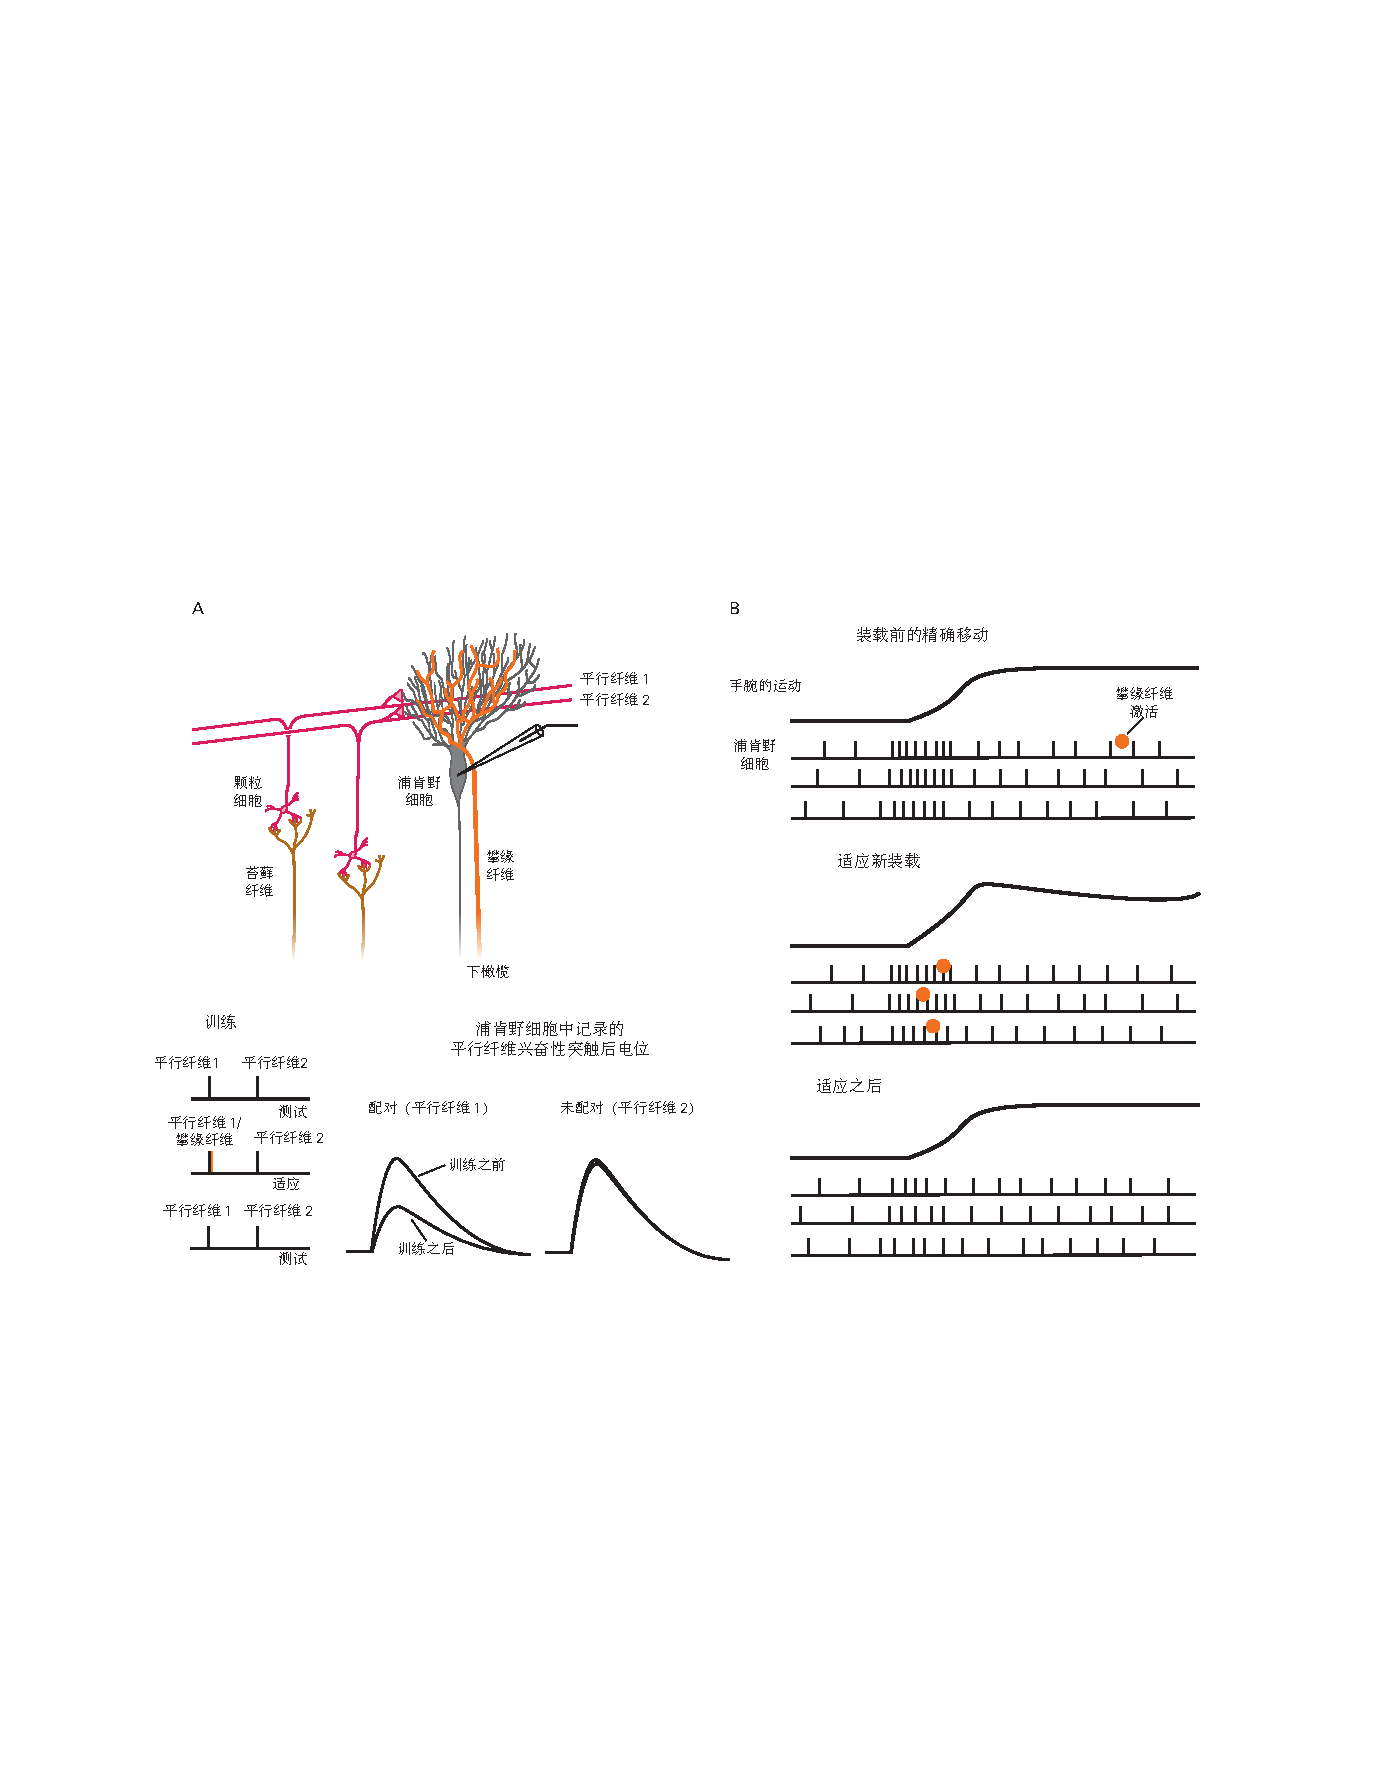
\includegraphics[width=0.9\linewidth]{chap37/fig_37_11}
	\caption{从平行纤维到浦肯野细胞突触输入的长期抑制是小脑学习的一种似是而非的机制。
		\textbf{A.} 两组不同的平行纤维和突触前攀爬纤维在体外受到电刺激。
		在攀爬纤维的同时重复刺激一组平行纤维 (PF1) 会长期降低这些平行纤维对后续刺激的反应。
		第二组平行纤维 (PF2) 的反应没有受到抑制,因为它们没有与突触前攀爬纤维同时受到刺激\cite{ito1982climbing}。
		\textbf{B.} 上图:猴子准确的手腕运动伴随着浦肯野细胞中的一阵简单尖峰脉冲,随后 后来在一次试验中释放了一根攀爬纤维。
		中:当猴子必须针对新的阻力(适应)做出相同的运动时,在每次试验的运动过程中都会发生攀爬纤维活动,并且运动本身会超过目标。
		底部:适应后,运动过程中简单尖峰的频率相当衰减,攀爬纤维在运动过程中或之后不活跃。
		如果小脑皮层的长期抑制在学习中发挥作用,这就是预期的事件顺序。
		攀爬纤维活动通常较低 (1/s),但在适应新负载期间会增加\cite{gilbert1977purkinje}。}
	\label{fig:37_11}
\end{figure}


许多针对各种运动学习系统的研究记录了浦肯野细胞的活动,这与小脑学习理论的预测一致。
例如,如果对训练有素的手臂运动施加了意想不到的阻力,则需要额外的肌肉张力才能运动。
在了解意外阻力之前,攀爬纤维活动可能会发出错误信号。
它们可能会抑制产生这些错误所涉及的平行纤维的突触强度,即那些在攀爬纤维活动时驱动浦肯野简单尖峰放电的纤维(图~\ref{fig:37_11}B)。
随着连续运动,传递有缺陷的中央命令的平行纤维输入越来越受到抑制,出现了更合适的简单尖峰活动模式,最终运动错误消失,同时出现了攀爬纤维错误信号。
这种结果虽然符合小脑学习理论,但并不能证明神经和行为学习是由平行纤维突触长期抑制浦肯野细胞引起的。



\subsection{在几种不同的运动系统中,小脑是运动学习所必需的}

小脑参与学习各种各样的运动,从肢体和眼球运动到行走。
在每个运动系统中,运动学习都会改善运动的前馈控制。
错误使电机控制暂时依赖于感官反馈,而电机学习可恢复理想情况,在这种情况下,性能是准确的,而不依赖于感官反馈。


依赖眼手协调的肢体运动适应可以通过让人们佩戴使光路偏向侧面的棱镜来证明。
当一个人戴着将整个视野向左移动的棱镜护目镜玩飞镖时,最初的飞镖投掷落在目标的左侧,其数量与棱镜的强度成正比。
主体通过练习逐渐适应失真;
在 10 到 30 次投掷后,飞镖会落在目标上(图 ~\ref{fig:37_12})。
当棱镜被移除时,适应仍然存在,飞镖击中目标右侧的距离与初始棱镜引起的误差大致相同。
小脑皮层或下橄榄受损的患者在此测试中严重受损或根本无法适应。


\begin{figure}[htbp]
	\centering
	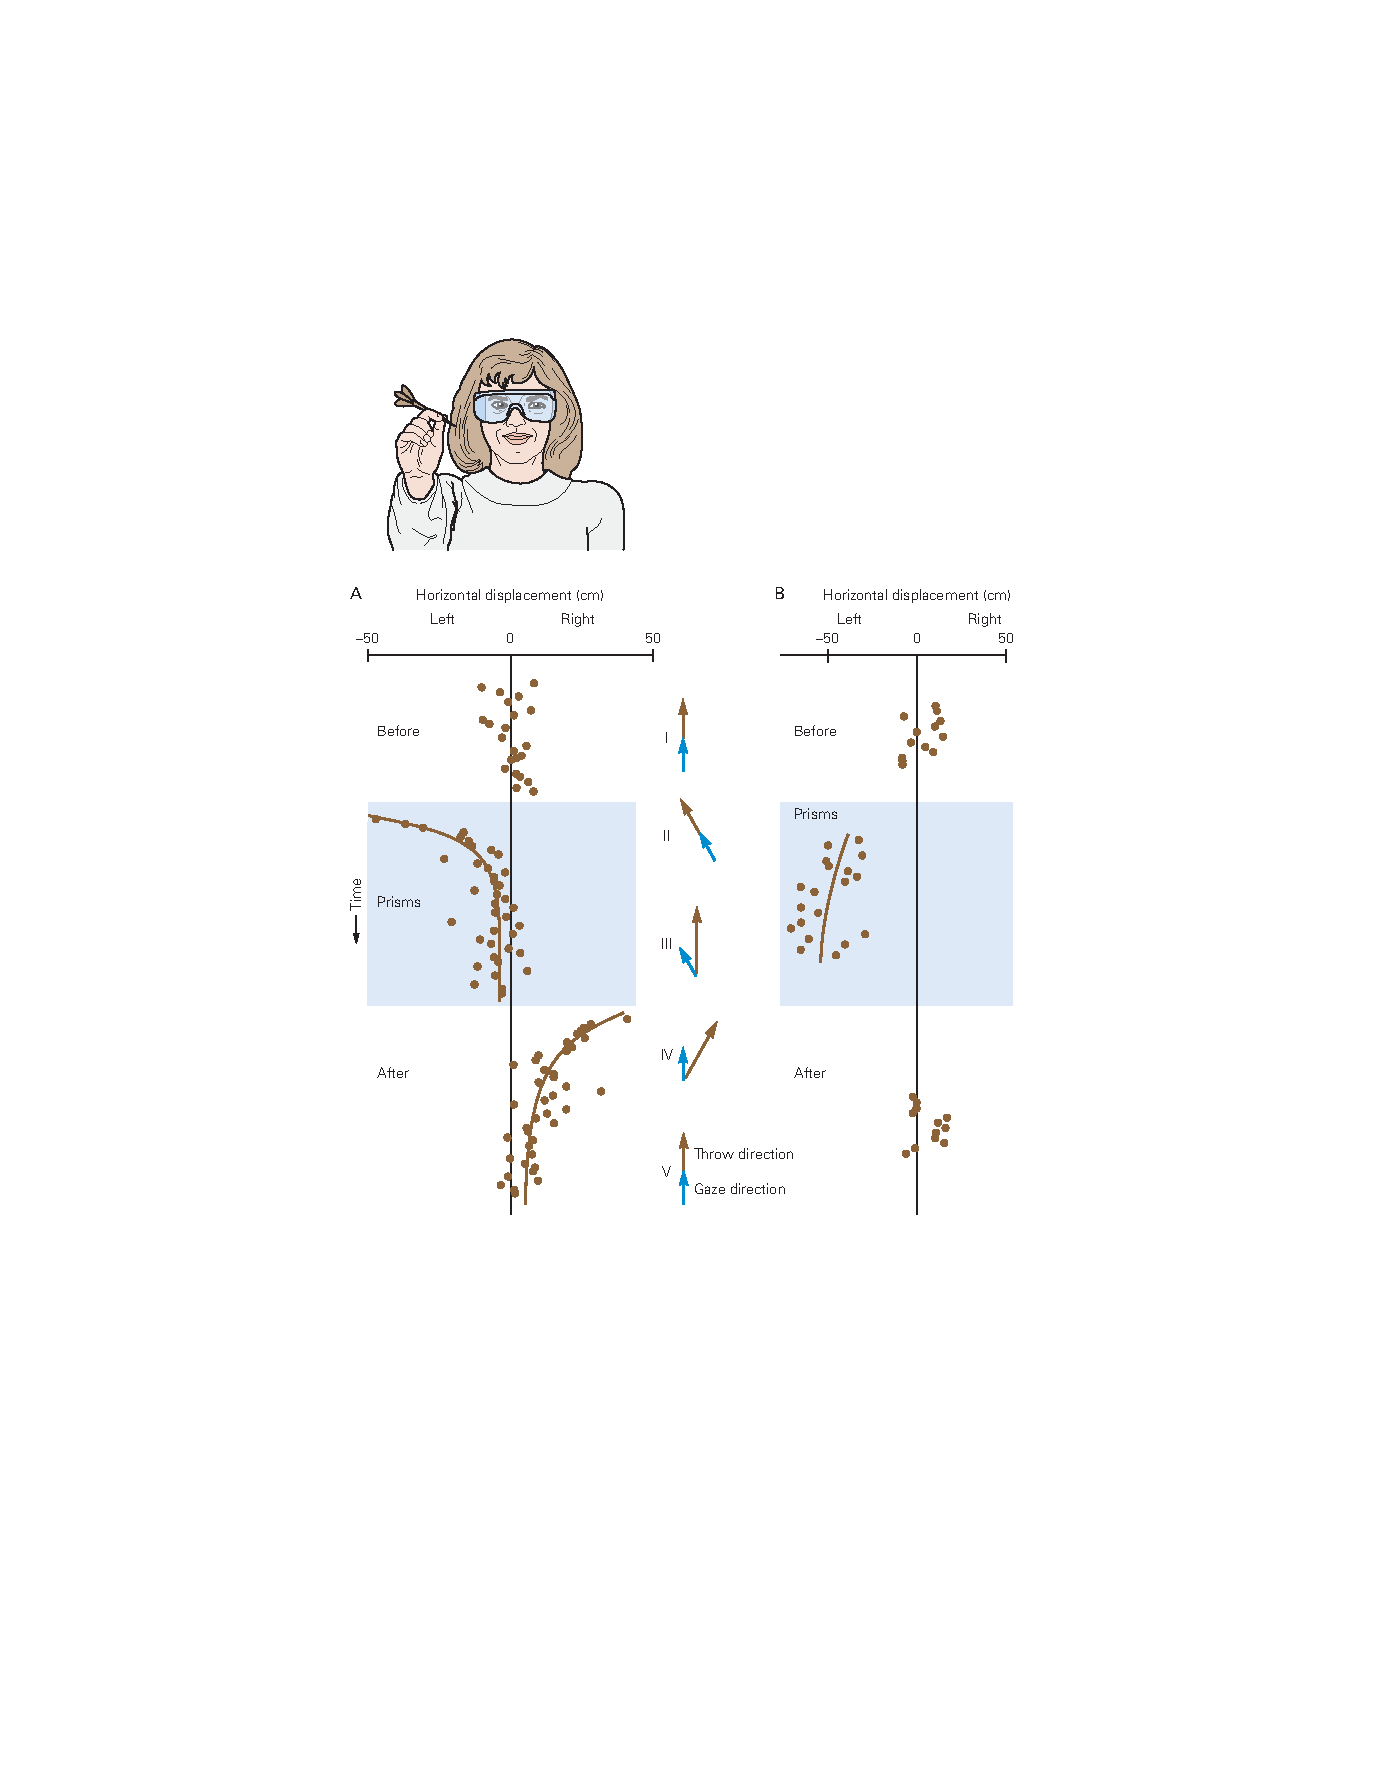
\includegraphics[width=0.75\linewidth]{chap37/fig_37_12}
	\caption{调整眼手协调以适应光学条件的变化。
		受试者佩戴棱镜护目镜,将光路向她的右侧弯曲。
		她必须沿着弯曲的光路向左看,才能看到正前方的目标\cite{martin1996throwing}。
		\textbf{A.} 在没有棱镜的情况下,受试者投掷的准确性很高 (I)。
		棱镜就位后的第一个击球位置偏左,因为手会投向眼睛所指向的位置。
		此后,从眼睛注视的地方向右击中目标 (II)。
		移除棱镜后,受试者将目光固定在目标的中心;
		第一次投掷命中中心右侧,远离眼睛指向的位置。
		此后,朝着目标 (III) 迈进。
		取下棱镜后,受试者立即将目光投向目标;
		她调整后的投掷是在注视方向的右侧和目标的右侧 (IV)。
		从适应中恢复过来后,她再次注视并向目标投掷(V)。
		棱镜使用期间和之后的数据符合指数曲线。
		注视和投掷方向分别由右侧的蓝色和棕色箭头表示。
		推断的凝视方向假定对象正在注视目标。
		\textbf{B.} 小脑后下动脉区域单侧梗死影响小脑下脚和小脑后外侧皮层的患者适应失败。}
	\label{fig:37_12}
\end{figure}


眨眼反应的经典调节也取决于完整的小脑。
在这种形式的联想学习中,一股空气直接吹向角膜,导致眼睛在中性刺激(例如音调)结束时眨眼。
如果音调和粉扑以固定的音调持续时间重复配对,那么大脑就会学习音调的预测能力,并且仅音调就足以引起眨眼。
Michael Mauk 和他的同事已经表明,大脑还可以了解刺激的时间,以便眨眼发生在正确的时间。
甚至可以学会在不同时间眨眼以响应不同频率的音调。


所有形式的共轭眼球运动都需要小脑才能正确执行,并且每种形式都需要涉及小脑的运动学习。
例如,当头部旋转时,前庭眼反射通常会使眼睛保持在目标上(第~\ref{chap:chap27}~章)。
头部在一个方向上的运动由前庭迷路感知,前庭迷路会启动相反方向的眼球运动,以防止视觉图像滑过视网膜。
当人类和实验动物佩戴改变视觉场景大小的眼镜时,前庭眼反射最初无法使图像在视网膜上保持稳定,因为反射的幅度不适合新条件。
然而,在连续佩戴眼镜几天后,反射的大小会逐渐减小(对于小型化眼镜)或增大(对于放大镜)(图 ~\ref{fig:37_13}A)。
需要进行这些更改以防止图像在视网膜上滑动,因为放大(或缩小)的图像也会移动得更快(或更慢)。
基线前庭眼反射的表现并不严重依赖于小脑,但它的适应性在实验动物中确实并且可以被称为絮状复合体的前庭小脑外侧部分的损伤所阻断。


\begin{figure}[htbp]
	\centering
	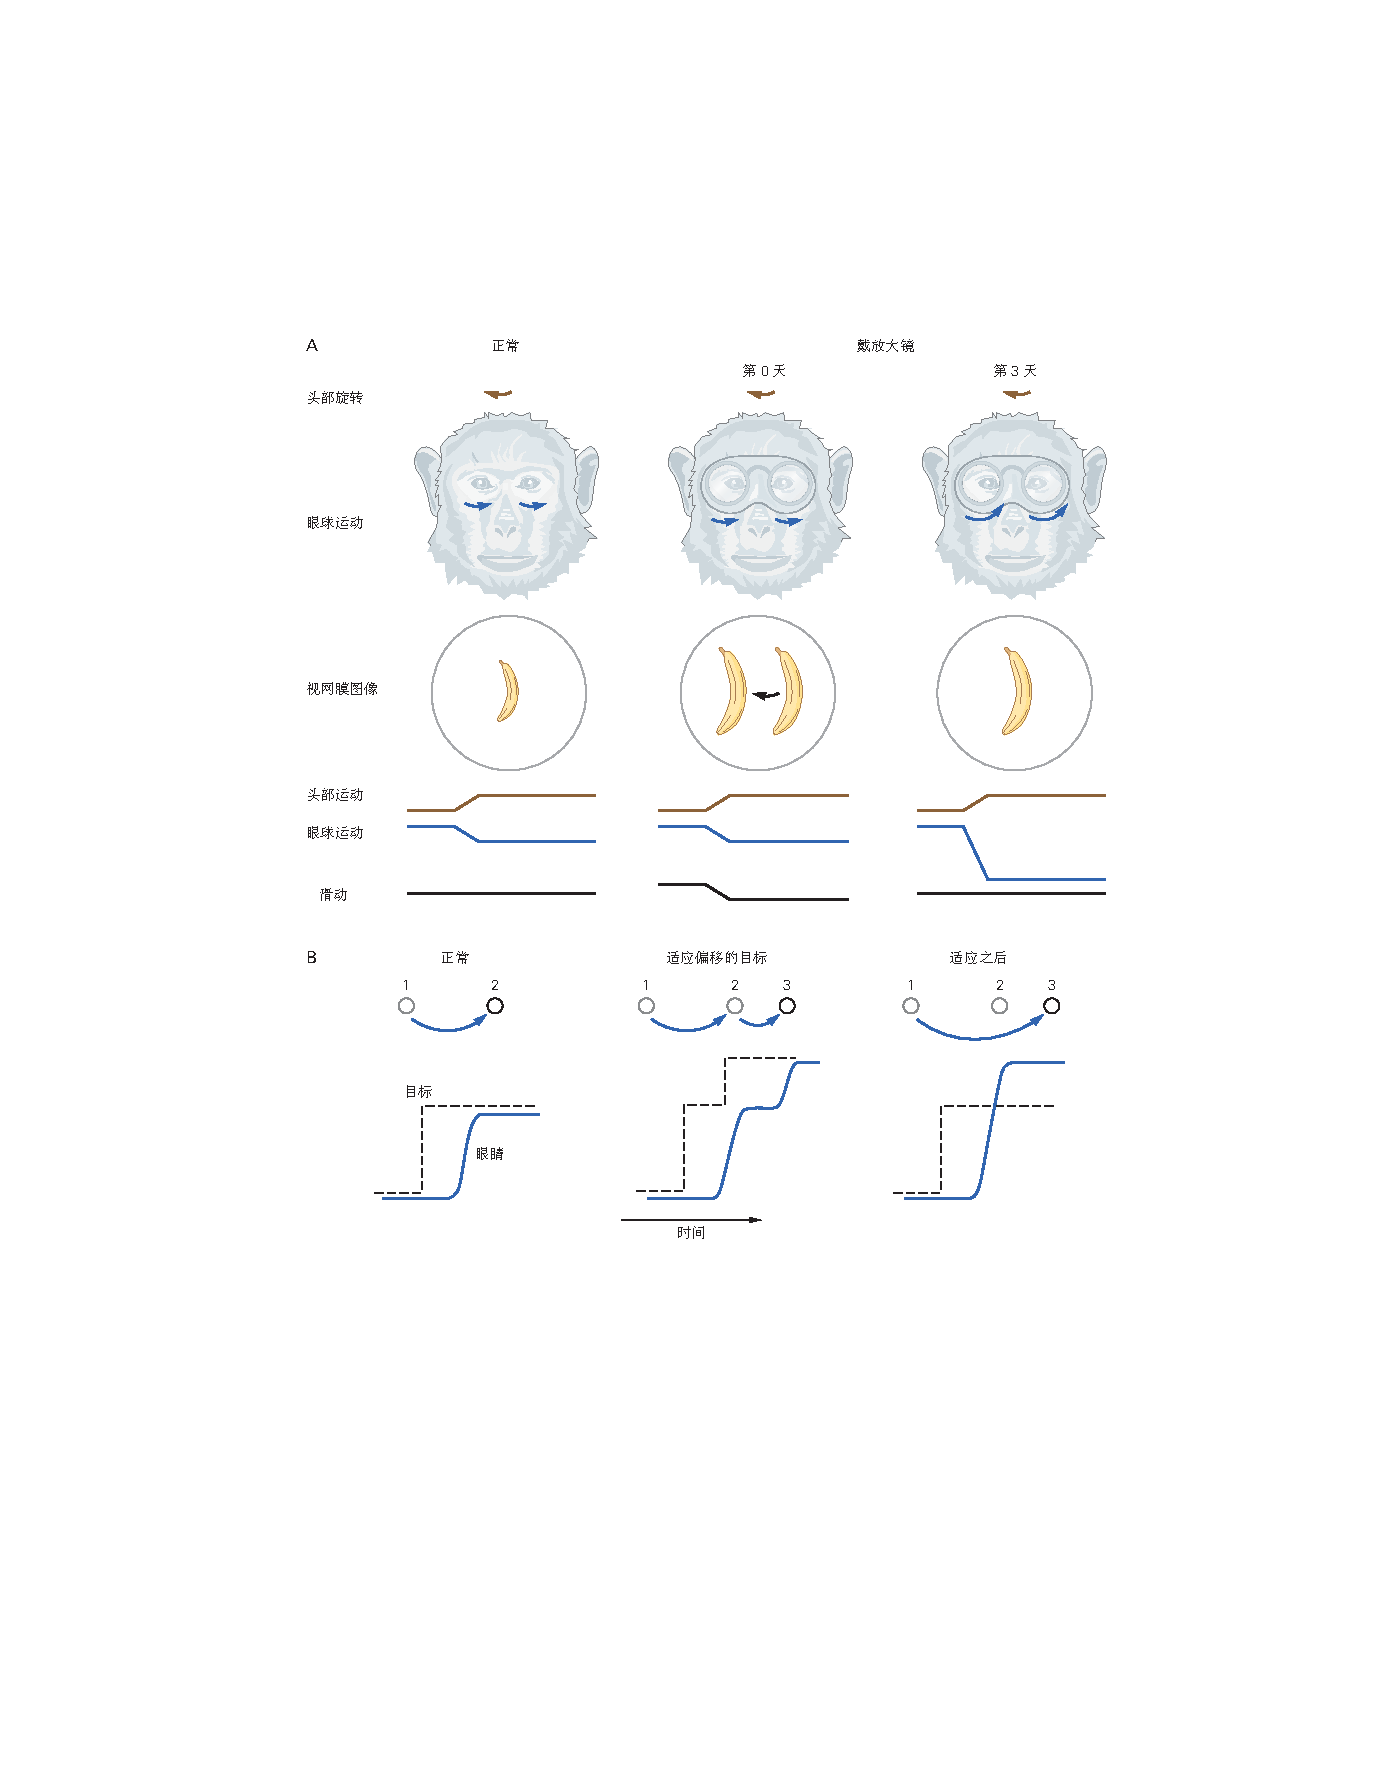
\includegraphics[width=0.8\linewidth]{chap37/fig_37_13}
	\caption{前庭-眼睛反射和扫视眼球运动中的小脑学习。
		\textbf{A.} 戴着放大镜的猴子前庭-眼睛反射的运动学习。这些列显示了学习前的正常情况,猴子第一次戴眼镜时的情况(第0天),以及完全适应后的情况(第一天)。
		睛的运动通常与转头相等且相反,在转头过程中香蕉在视网膜中保持稳定。
		戴上眼镜,香蕉看起来更大了;
		当头部转动时,前庭-眼睛反射太小,香蕉的图像滑过视网膜。
		适应后,眼睛的运动足够大,以至于在转头时香蕉的图像在视网膜上再次保持稳定\cite{lisberger1988neural}。)
		\textbf{B.} 扫视眼动中的运动学习。这些列显示了在正常条件下、第一次适应试验和完全适应后的扫视。
		通常,扫视通过将眼睛几乎完美地带到新的目标位置来响应目标位置的变化。
		在适应过程中,目标在初始扫视过程中移动到新的位置,需要第二次扫视才能将眼睛带到新的最终目标位置。
		在适应之后,原始目标位置唤起更大的扫视,即使目标没有移动,也适合将眼睛带到新的目标位置。}
	\label{fig:37_13}
\end{figure}


眼球扫视运动还取决于小叶 V、VI 和 VII 中动眼\textit{小脑蚓体}浦肯野细胞的完整性(图~\ref{fig:37_2}C)。
这些细胞在眼跳之前和期间放电,\textit{小脑蚓体}的损伤会导致眼跳过度,就像我们在小脑患者的手臂运动中看到的那样。
与眼跳有关的\textit{小脑蚓体}神经元的输出通过尾部顶核的一个非常小的区域传输到网状结构中的眼跳发生器。


相同的浦肯野细胞参与一种称为扫视适应的运动学习形式。
通过让猴子注视前方的目标然后在偏心位置显示新目标来证明这种适应。
在对新目标的扫视过程中,实验者将新目标移动到更偏心的位置。
最初,受试者需要进行第二次扫视以注视目标。
逐渐地,经过数百次试验,第一个扫视的振幅逐渐增加,从而将眼睛直接带到目标的最终位置(图~\ref{fig:37_13}B)。
扫视适应过程中的记录表明,在学习过程中,攀爬纤维输入到动眼\textit{小脑蚓体}的浦肯野细胞会发出扫视错误信号,并且同一细胞的单棘放电率会随着猴子的眼球运动而逐渐适应。
因此,动眼\textit{小脑蚓体}可能是运动学习扫视眼球运动幅度的部位。
这个故事对于平滑跟随眼球运动非常相似,除了小脑的相关部分是絮状复合体,使用参与前庭眼反射适应的相同浦肯野细胞。


最后,已经在小脑患者中使用要求一条腿比另一条腿移动得更快的分带式跑步机研究了新步行模式的学习。
当两种跑带速度不同时,小脑损伤不会影响使用反馈立即改变步行模式的能力:
患者可以延长他们站在较慢跑带上的时间,并缩短他们站在较快跑带上的时间。
然而,小脑病患者无法学习数百步以使其行走模式对称,而健康人则可以(见图~\ref{fig:30_14})。



\subsection{学习发生在小脑的几个部位}

我们现在知道小脑微回路中有许多突触和细胞可塑性位点。
几乎每个已研究的突触都会经历增强或抑制,小脑学习理论也相应地得到了扩展。
对小脑回路在运动学习中的作用的详细分析已在几个运动系统中进行:
多种眼球运动的适应、眨眼的经典条件反射和手臂运动中的运动学习。


在当今小脑学习的扩展理论中,学习不仅发生在小脑皮层,如\textit{马尔}、Albus 和 Ito 所假设的,而且还发生在小脑深部核团(图~\ref{fig:37_14})。
我们对小脑皮层学习的理解部分基于从平行纤维到浦肯野细胞的突触的长期抑制,但许多其他突触具有可塑性,它们也可能参与其中。
现有证据仍然与长期存在的观点相一致,即来自攀爬纤维的输入提供了导致小脑皮层内突触强度变化的主要指导信号,但现在也有其他指导信号的可能性。
学习可能来自多个位点的协调突触可塑性,而不是来自单个位点的变化。


\begin{figure}[htbp]
	\centering
	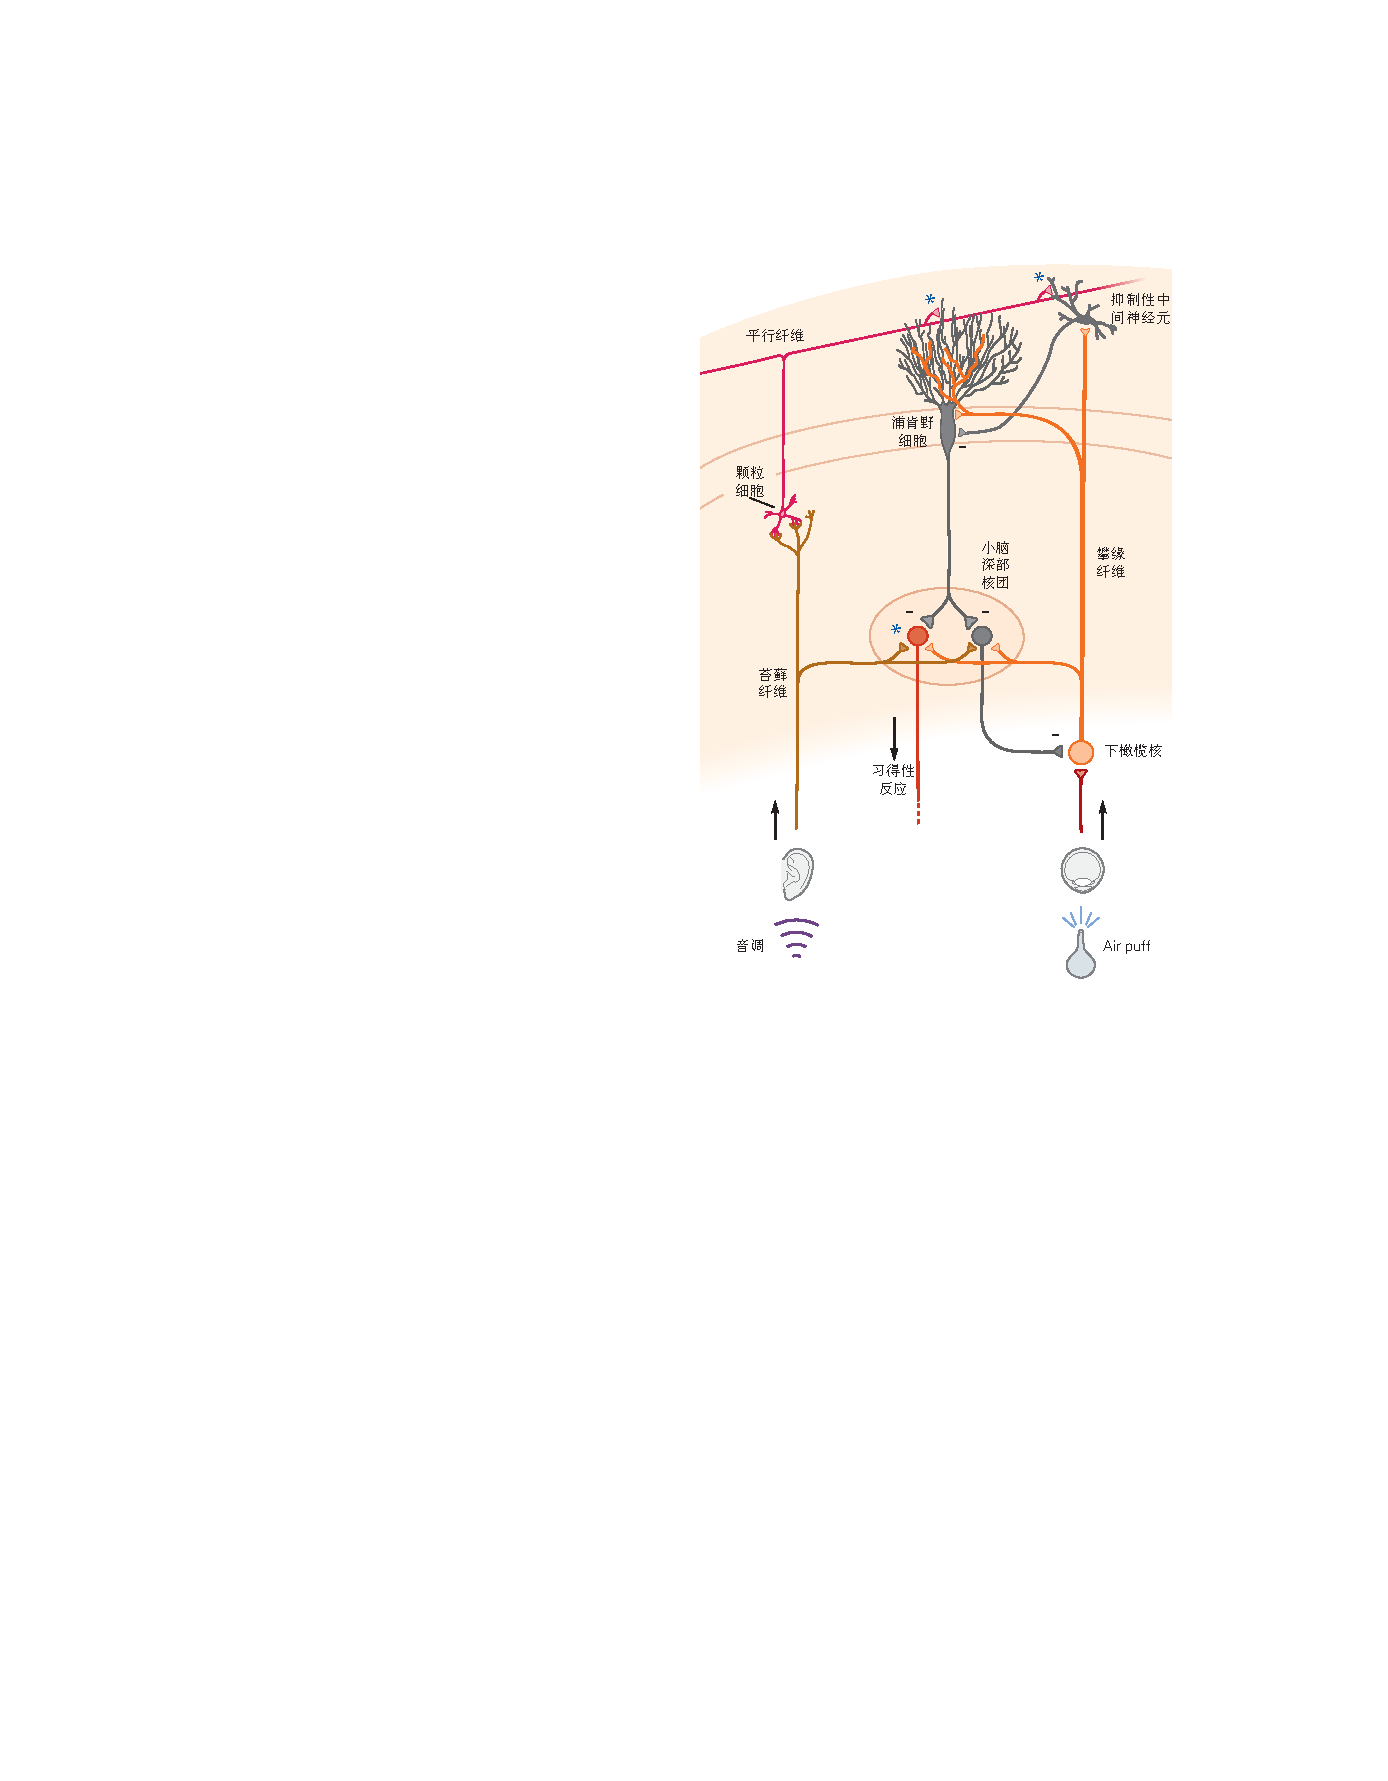
\includegraphics[width=0.5\linewidth]{chap37/fig_37_14}
	\caption{小脑微回路中的学习可以发生在小脑皮层和\textit{小脑深部核团}中。
		该图基于经典的眨眼条件反射,由\textit{音调}(所谓的由\textit{苔藓纤维}携带的条件刺激)和喷气(由\textit{攀爬纤维}携带的无条件刺激)配对驱动。
		当\textit{攀爬纤维}和\textit{平行纤维}一起活跃时,学习发生在\textit{平行纤维-浦肯野细胞}突触处。
		学习也发生在小脑深核的苔藓纤维突触处。
		(学习地点用星号表示。)
		虽然这个例子描绘了一个经典的调节范式,但当头部转动与视网膜上的图像运动相关时,可塑性发生在前庭眼反射适应过程中的相同位置(第~\ref{chap:chap27}~章)\cite{carey2002embarrassed}。}
	\label{fig:37_14}
\end{figure}


对眨眼的经典条件反射和前庭眼反射的适应性的研究提供了强有力的证据,表明学习发生在小脑皮层和小脑深部核团中。
此外,大量证据表明,学习可能首先发生在小脑皮层,然后转移到小脑深部核团。
至少对于眨眼调节,小脑皮层可能在学习时间方面发挥特殊作用。


如前所述,小脑利用内部模型来确保在感觉反馈的任何引导之前平稳准确地运动。
导致回路学习的突触变化可能是创建和维护准确内部模型的机制。
小脑学习的一项重要功能可能是不断调整内部模型。
小脑内部模型可以使用感觉反馈来调整突触和细胞功能,以便运动指令产生快速、准确和平稳的运动。
因此,小脑似乎是最早研究者设想的学习机器,但其学习能力可能比最初想象的更强大、分布更广,并可能影响所有小脑对行为的贡献。



\section{要点}

1. 小脑在运动中起着至关重要的作用。
小脑损伤会导致严重的运动不协调,称为共济失调,它会影响从眼睛和肢体运动到平衡和行走的所有运动。
小脑损伤也会导致一些感觉缺陷,但仅限于主动运动期间。


2. 小脑还在认知和情绪行为中发挥作用。
这些领域的缺陷在小脑损伤后不太明显,但会在正式测试中出现。
运动和非运动领域的缺陷可能有一个共同的机制,但该机制尚不清楚。


3. 小脑通过与其他大脑结构的连接发挥作用。
它的输入间接来自大脑皮层的广泛区域,以及脑干和脊髓。
小脑输出投射到前庭核团、脑干网状结构和红核,并通过丘脑投射到大脑皮层的广泛区域。


4. 小脑和大脑皮层之间的相互联系包括感觉和运动皮层以及顶叶和前额叶皮层的广泛区域。
小脑连接被组织为一系列平行的、闭合的、循环的回路,其中大脑皮层的给定区域与小脑的给定部分同时进行传出和传入连接。


5. 小脑皮层的回路是高度刻板的,这表明它与其他大脑区域的相互作用具有共同的计算机制。
它包括一个输入颗粒层,其中颗粒细胞上的苔藓纤维突触和高尔基细胞提供抑制反馈;
抑制性浦肯野细胞层,具有小脑皮层的唯一输出神经元;
和一个分子层,浦肯野细胞树突和抑制性中间神经元从颗粒细胞轴突出现的平行纤维接收输入。


6. 小脑的攀缘纤维和苔藓纤维输入在解剖学上非常不同。
每个浦肯野细胞从单个攀缘纤维接收许多突触接触,但可以通过颗粒细胞受到大量苔藓纤维的影响。
攀爬纤维以非常低的频率发射并在浦肯野细胞中引起单一的“复杂尖峰”。
苔藓纤维会产生“简单的尖峰”,可以以非常高的速率放电。
人们认为这些输入之间的相互作用对于学习是必不可少的。


7. 小脑运动控制理论强调几个一般原则。
在有用的感觉反馈发生之前,小脑对于产生可靠的前馈动作很重要。
它在计时的内部控制中起着关键作用。
小脑依赖于将感官输入与报告所命令的运动的必然放电相结合的计算。
运动效应器器官和世界的内部模型允许小脑估计运动系统的状态并指导准确的前馈动作。


8. 运动的学习和适应是小脑的基本功能。
小脑学习需要有关运动错误的反馈,并在逐个试验的基础上更新运动。
小脑中有许多突触可塑性位点,目前运动学习系统的证据支持小脑中至少有两个学习位点。
一个部位涉及从平行纤维到浦肯野细胞的突触长期抑制,由攀爬纤维输入发出的错误信号引导。
另一个位点位于小脑深部核团。
很可能相同的学习机制用于认知和情绪处理。



